\documentclass[1p]{elsarticle_modified}
%\bibliographystyle{elsarticle-num}

%\usepackage[colorlinks]{hyperref}
%\usepackage{abbrmath_seonhwa} %\Abb, \Ascr, \Acal ,\Abf, \Afrak
\usepackage{amsfonts}
\usepackage{amssymb}
\usepackage{amsmath}
\usepackage{amsthm}
\usepackage{scalefnt}
\usepackage{amsbsy}
\usepackage{kotex}
\usepackage{caption}
\usepackage{subfig}
\usepackage{color}
\usepackage{graphicx}
\usepackage{xcolor} %% white, black, red, green, blue, cyan, magenta, yellow
\usepackage{float}
\usepackage{setspace}
\usepackage{hyperref}

\usepackage{tikz}
\usetikzlibrary{arrows}

\usepackage{multirow}
\usepackage{array} % fixed length table
\usepackage{hhline}

%%%%%%%%%%%%%%%%%%%%%
\makeatletter
\renewcommand*\env@matrix[1][\arraystretch]{%
	\edef\arraystretch{#1}%
	\hskip -\arraycolsep
	\let\@ifnextchar\new@ifnextchar
	\array{*\c@MaxMatrixCols c}}
\makeatother %https://tex.stackexchange.com/questions/14071/how-can-i-increase-the-line-spacing-in-a-matrix
%%%%%%%%%%%%%%%

\usepackage[normalem]{ulem}

\newcommand{\msout}[1]{\ifmmode\text{\sout{\ensuremath{#1}}}\else\sout{#1}\fi}
%SOURCE: \msout is \stkout macro in https://tex.stackexchange.com/questions/20609/strikeout-in-math-mode

\newcommand{\cancel}[1]{
	\ifmmode
	{\color{red}\msout{#1}}
	\else
	{\color{red}\sout{#1}}
	\fi
}

\newcommand{\add}[1]{
	{\color{blue}\uwave{#1}}
}

\newcommand{\replace}[2]{
	\ifmmode
	{\color{red}\msout{#1}}{\color{blue}\uwave{#2}}
	\else
	{\color{red}\sout{#1}}{\color{blue}\uwave{#2}}
	\fi
}

\newcommand{\Sol}{\mathcal{S}} %segment
\newcommand{\D}{D} %diagram
\newcommand{\A}{\mathcal{A}} %arc


%%%%%%%%%%%%%%%%%%%%%%%%%%%%%5 test

\def\sl{\operatorname{\textup{SL}}(2,\Cbb)}
\def\psl{\operatorname{\textup{PSL}}(2,\Cbb)}
\def\quan{\mkern 1mu \triangleright \mkern 1mu}

\theoremstyle{definition}
\newtheorem{thm}{Theorem}[section]
\newtheorem{prop}[thm]{Proposition}
\newtheorem{lem}[thm]{Lemma}
\newtheorem{ques}[thm]{Question}
\newtheorem{cor}[thm]{Corollary}
\newtheorem{defn}[thm]{Definition}
\newtheorem{exam}[thm]{Example}
\newtheorem{rmk}[thm]{Remark}
\newtheorem{alg}[thm]{Algorithm}

\newcommand{\I}{\sqrt{-1}}
\begin{document}

%\begin{frontmatter}
%
%\title{Boundary parabolic representations of knots up to 8 crossings}
%
%%% Group authors per affiliation:
%\author{Yunhi Cho} 
%\address{Department of Mathematics, University of Seoul, Seoul, Korea}
%\ead{yhcho@uos.ac.kr}
%
%
%\author{Seonhwa Kim} %\fnref{s_kim}}
%\address{Center for Geometry and Physics, Institute for Basic Science, Pohang, 37673, Korea}
%\ead{ryeona17@ibs.re.kr}
%
%\author{Hyuk Kim}
%\address{Department of Mathematical Sciences, Seoul National University, Seoul 08826, Korea}
%\ead{hyukkim@snu.ac.kr}
%
%\author{Seokbeom Yoon}
%\address{Department of Mathematical Sciences, Seoul National University, Seoul, 08826,  Korea}
%\ead{sbyoon15@snu.ac.kr}
%
%\begin{abstract}
%We find all boundary parabolic representation of knots up to 8 crossings.
%
%\end{abstract}
%\begin{keyword}
%    \MSC[2010] 57M25 
%\end{keyword}
%
%\end{frontmatter}

%\linenumbers
%\tableofcontents
%
\newcommand\colored[1]{\textcolor{white}{\rule[-0.35ex]{0.8em}{1.4ex}}\kern-0.8em\color{red} #1}%
%\newcommand\colored[1]{\textcolor{white}{ #1}\kern-2.17ex	\textcolor{white}{ #1}\kern-1.81ex	\textcolor{white}{ #1}\kern-2.15ex\color{red}#1	}

{\Large $\underline{12a_{0695}~(K12a_{0695})}$}

\setlength{\tabcolsep}{10pt}
\renewcommand{\arraystretch}{1.6}
\vspace{1cm}\begin{tabular}{m{100pt}>{\centering\arraybackslash}m{274pt}}
\multirow{5}{120pt}{
	\centering
	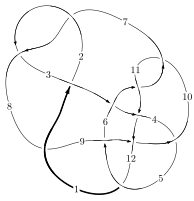
\includegraphics[width=112pt]{../../../GIT/diagram.site/Diagrams/png/1496_12a_0695.png}\\
\ \ \ A knot diagram\footnotemark}&
\allowdisplaybreaks
\textbf{Linearized knot diagam} \\
\cline{2-2}
 &
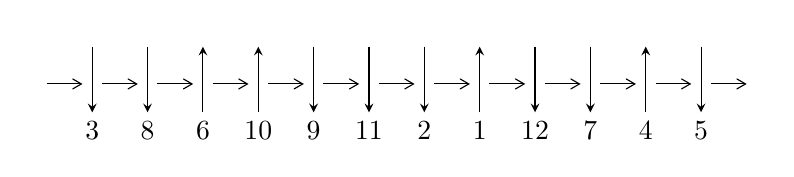
\begin{tikzpicture}[x=20pt, y=17pt]
	% nodes
	\node (C0) at (0, 0) {};
	\node (C1) at (1, 0) {};
	\node (C1U) at (1, +1) {};
	\node (C1D) at (1, -1) {3};

	\node (C2) at (2, 0) {};
	\node (C2U) at (2, +1) {};
	\node (C2D) at (2, -1) {8};

	\node (C3) at (3, 0) {};
	\node (C3U) at (3, +1) {};
	\node (C3D) at (3, -1) {6};

	\node (C4) at (4, 0) {};
	\node (C4U) at (4, +1) {};
	\node (C4D) at (4, -1) {10};

	\node (C5) at (5, 0) {};
	\node (C5U) at (5, +1) {};
	\node (C5D) at (5, -1) {9};

	\node (C6) at (6, 0) {};
	\node (C6U) at (6, +1) {};
	\node (C6D) at (6, -1) {11};

	\node (C7) at (7, 0) {};
	\node (C7U) at (7, +1) {};
	\node (C7D) at (7, -1) {2};

	\node (C8) at (8, 0) {};
	\node (C8U) at (8, +1) {};
	\node (C8D) at (8, -1) {1};

	\node (C9) at (9, 0) {};
	\node (C9U) at (9, +1) {};
	\node (C9D) at (9, -1) {12};

	\node (C10) at (10, 0) {};
	\node (C10U) at (10, +1) {};
	\node (C10D) at (10, -1) {7};

	\node (C11) at (11, 0) {};
	\node (C11U) at (11, +1) {};
	\node (C11D) at (11, -1) {4};

	\node (C12) at (12, 0) {};
	\node (C12U) at (12, +1) {};
	\node (C12D) at (12, -1) {5};
	\node (C13) at (13, 0) {};

	% arrows
	\draw[->,>={angle 60}]
	(C0) edge (C1) (C1) edge (C2) (C2) edge (C3) (C3) edge (C4) (C4) edge (C5) (C5) edge (C6) (C6) edge (C7) (C7) edge (C8) (C8) edge (C9) (C9) edge (C10) (C10) edge (C11) (C11) edge (C12) (C12) edge (C13) ;	\draw[->,>=stealth]
	(C1U) edge (C1D) (C2U) edge (C2D) (C3D) edge (C3U) (C4D) edge (C4U) (C5U) edge (C5D) (C6U) edge (C6D) (C7U) edge (C7D) (C8D) edge (C8U) (C9U) edge (C9D) (C10U) edge (C10D) (C11D) edge (C11U) (C12U) edge (C12D) ;
	\end{tikzpicture} \\
\hhline{~~} \\& 
\textbf{Solving Sequence} \\ \cline{2-2} 
 &
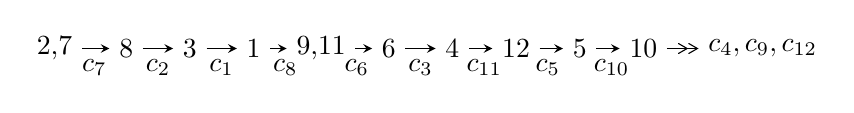
\begin{tikzpicture}[x=23pt, y=7pt]
	% node
	\node (A0) at (-1/8, 0) {2,7};
	\node (A1) at (1, 0) {8};
	\node (A2) at (2, 0) {3};
	\node (A3) at (3, 0) {1};
	\node (A4) at (65/16, 0) {9,11};
	\node (A5) at (41/8, 0) {6};
	\node (A6) at (49/8, 0) {4};
	\node (A7) at (57/8, 0) {12};
	\node (A8) at (65/8, 0) {5};
	\node (A9) at (73/8, 0) {10};
	\node (C1) at (1/2, -1) {$c_{7}$};
	\node (C2) at (3/2, -1) {$c_{2}$};
	\node (C3) at (5/2, -1) {$c_{1}$};
	\node (C4) at (7/2, -1) {$c_{8}$};
	\node (C5) at (37/8, -1) {$c_{6}$};
	\node (C6) at (45/8, -1) {$c_{3}$};
	\node (C7) at (53/8, -1) {$c_{11}$};
	\node (C8) at (61/8, -1) {$c_{5}$};
	\node (C9) at (69/8, -1) {$c_{10}$};
	\node (A10) at (11, 0) {$c_{4},c_{9},c_{12}$};

	% edge
	\draw[->,>=stealth]	
	(A0) edge (A1) (A1) edge (A2) (A2) edge (A3) (A3) edge (A4) (A4) edge (A5) (A5) edge (A6) (A6) edge (A7) (A7) edge (A8) (A8) edge (A9) ;
	\draw[->>,>={angle 60}]	
	(A9) edge (A10);
\end{tikzpicture} \\ 

\end{tabular} \\

\footnotetext{
The image of knot diagram is generated by the software ``\textbf{Draw programme}" developed by Andrew Bartholomew(\url{http://www.layer8.co.uk/maths/draw/index.htm\#Running-draw}), where we modified some parts for our purpose(\url{https://github.com/CATsTAILs/LinksPainter}).
}\phantom \\ \newline 
\centering \textbf{Ideals for irreducible components\footnotemark of $X_{\text{par}}$} 
 
\begin{align*}
I^u_{1}&=\langle 
-8.05911\times10^{332} u^{175}+4.18234\times10^{332} u^{174}+\cdots+1.15862\times10^{331} b-1.72139\times10^{333},\\
\phantom{I^u_{1}}&\phantom{= \langle  }4.55348\times10^{333} u^{175}-2.30916\times10^{333} u^{174}+\cdots+1.15862\times10^{331} a+9.31822\times10^{333},\;u^{176}- u^{175}+\cdots+u-1\rangle \\
I^u_{2}&=\langle 
-1320 u^{38}+288 u^{37}+\cdots+79 b-520,\;-1681 u^{38}+1253 u^{37}+\cdots+79 a-2010,\\
\phantom{I^u_{2}}&\phantom{= \langle  }u^{39}-11 u^{37}+\cdots-7 u^2+1\rangle \\
\\
\end{align*}
\raggedright * 2 irreducible components of $\dim_{\mathbb{C}}=0$, with total 215 representations.\\
\footnotetext{All coefficients of polynomials are rational numbers. But the coefficients are sometimes approximated in decimal forms when there is not enough margin.}
\newpage
\renewcommand{\arraystretch}{1}
\centering \section*{I. $I^u_{1}= \langle -8.06\times10^{332} u^{175}+4.18\times10^{332} u^{174}+\cdots+1.16\times10^{331} b-1.72\times10^{333},\;4.55\times10^{333} u^{175}-2.31\times10^{333} u^{174}+\cdots+1.16\times10^{331} a+9.32\times10^{333},\;u^{176}- u^{175}+\cdots+u-1 \rangle$}
\flushleft \textbf{(i) Arc colorings}\\
\begin{tabular}{m{7pt} m{180pt} m{7pt} m{180pt} }
\flushright $a_{2}=$&$\begin{pmatrix}0\\u\end{pmatrix}$ \\
\flushright $a_{7}=$&$\begin{pmatrix}1\\0\end{pmatrix}$ \\
\flushright $a_{8}=$&$\begin{pmatrix}1\\u^2\end{pmatrix}$ \\
\flushright $a_{3}=$&$\begin{pmatrix}- u\\- u^3+u\end{pmatrix}$ \\
\flushright $a_{1}=$&$\begin{pmatrix}u^3\\u^5- u^3+u\end{pmatrix}$ \\
\flushright $a_{9}=$&$\begin{pmatrix}u^6- u^4+1\\u^8-2 u^6+2 u^4\end{pmatrix}$ \\
\flushright $a_{11}=$&$\begin{pmatrix}-393.011 u^{175}+199.304 u^{174}+\cdots-813.604 u-804.255\\69.5581 u^{175}-36.0978 u^{174}+\cdots+168.780 u+148.573\end{pmatrix}$ \\
\flushright $a_{6}=$&$\begin{pmatrix}80.7532 u^{175}-51.9642 u^{174}+\cdots+340.506 u+219.915\\-61.1617 u^{175}+32.3738 u^{174}+\cdots-165.021 u-130.889\end{pmatrix}$ \\
\flushright $a_{4}=$&$\begin{pmatrix}142.500 u^{175}-69.2550 u^{174}+\cdots+214.426 u+268.079\\-25.5883 u^{175}+11.5078 u^{174}+\cdots-41.3361 u-48.0003\end{pmatrix}$ \\
\flushright $a_{12}=$&$\begin{pmatrix}-130.167 u^{175}+63.4849 u^{174}+\cdots-188.976 u-239.495\\46.1287 u^{175}-22.1889 u^{174}+\cdots+93.4806 u+91.9512\end{pmatrix}$ \\
\flushright $a_{5}=$&$\begin{pmatrix}23.0458 u^{175}-20.8010 u^{174}+\cdots+171.101 u+93.5464\\-65.4961 u^{175}+34.4807 u^{174}+\cdots-174.631 u-139.424\end{pmatrix}$ \\
\flushright $a_{10}=$&$\begin{pmatrix}-323.452 u^{175}+163.206 u^{174}+\cdots-644.825 u-655.682\\69.5581 u^{175}-36.0978 u^{174}+\cdots+168.780 u+148.573\end{pmatrix}$\\&\end{tabular}
\flushleft \textbf{(ii) Obstruction class $= -1$}\\~\\
\flushleft \textbf{(iii) Cusp Shapes $= 392.821 u^{175}-202.925 u^{174}+\cdots+886.971 u+824.892$}\\~\\
\newpage\renewcommand{\arraystretch}{1}
\flushleft \textbf{(iv) u-Polynomials at the component}\newline \\
\begin{tabular}{m{50pt}|m{274pt}}
Crossings & \hspace{64pt}u-Polynomials at each crossing \\
\hline $$\begin{aligned}c_{1}\end{aligned}$$&$\begin{aligned}
&u^{176}+91 u^{175}+\cdots+15 u+1
\end{aligned}$\\
\hline $$\begin{aligned}c_{2},c_{7}\end{aligned}$$&$\begin{aligned}
&u^{176}- u^{175}+\cdots+u-1
\end{aligned}$\\
\hline $$\begin{aligned}c_{3}\end{aligned}$$&$\begin{aligned}
&u^{176}-7 u^{175}+\cdots-6680352 u-155647
\end{aligned}$\\
\hline $$\begin{aligned}c_{4}\end{aligned}$$&$\begin{aligned}
&u^{176}+u^{175}+\cdots-2208 u+2592
\end{aligned}$\\
\hline $$\begin{aligned}c_{5}\end{aligned}$$&$\begin{aligned}
&u^{176}+4 u^{175}+\cdots-28 u+1
\end{aligned}$\\
\hline $$\begin{aligned}c_{6},c_{10}\end{aligned}$$&$\begin{aligned}
&u^{176}+48 u^{174}+\cdots+26878 u+31907
\end{aligned}$\\
\hline $$\begin{aligned}c_{8}\end{aligned}$$&$\begin{aligned}
&u^{176}-6 u^{175}+\cdots+22634157 u-2052171
\end{aligned}$\\
\hline $$\begin{aligned}c_{9}\end{aligned}$$&$\begin{aligned}
&u^{176}-15 u^{175}+\cdots+55 u-1
\end{aligned}$\\
\hline $$\begin{aligned}c_{11}\end{aligned}$$&$\begin{aligned}
&u^{176}+3 u^{175}+\cdots-39223 u+39029
\end{aligned}$\\
\hline $$\begin{aligned}c_{12}\end{aligned}$$&$\begin{aligned}
&u^{176}+2 u^{175}+\cdots+58430 u-7292
\end{aligned}$\\
\hline
\end{tabular}\\~\\
\newpage\renewcommand{\arraystretch}{1}
\flushleft \textbf{(v) Riley Polynomials at the component}\newline \\
\begin{tabular}{m{50pt}|m{274pt}}
Crossings & \hspace{64pt}Riley Polynomials at each crossing \\
\hline $$\begin{aligned}c_{1}\end{aligned}$$&$\begin{aligned}
&y^{176}+y^{175}+\cdots-87 y+1
\end{aligned}$\\
\hline $$\begin{aligned}c_{2},c_{7}\end{aligned}$$&$\begin{aligned}
&y^{176}-91 y^{175}+\cdots-15 y+1
\end{aligned}$\\
\hline $$\begin{aligned}c_{3}\end{aligned}$$&$\begin{aligned}
&y^{176}-23 y^{175}+\cdots-30510996087262 y+24225988609
\end{aligned}$\\
\hline $$\begin{aligned}c_{4}\end{aligned}$$&$\begin{aligned}
&y^{176}+y^{175}+\cdots+583363584 y+6718464
\end{aligned}$\\
\hline $$\begin{aligned}c_{5}\end{aligned}$$&$\begin{aligned}
&y^{176}-26 y^{175}+\cdots+92 y+1
\end{aligned}$\\
\hline $$\begin{aligned}c_{6},c_{10}\end{aligned}$$&$\begin{aligned}
&y^{176}+96 y^{175}+\cdots+33870568190 y+1018056649
\end{aligned}$\\
\hline $$\begin{aligned}c_{8}\end{aligned}$$&$\begin{aligned}
&y^{176}+74 y^{175}+\cdots-184259306568177 y+4211405813241
\end{aligned}$\\
\hline $$\begin{aligned}c_{9}\end{aligned}$$&$\begin{aligned}
&y^{176}+9 y^{175}+\cdots-417 y+1
\end{aligned}$\\
\hline $$\begin{aligned}c_{11}\end{aligned}$$&$\begin{aligned}
&y^{176}-41 y^{175}+\cdots-26665548103 y+1523262841
\end{aligned}$\\
\hline $$\begin{aligned}c_{12}\end{aligned}$$&$\begin{aligned}
&y^{176}-32 y^{175}+\cdots-4059654828 y+53173264
\end{aligned}$\\
\hline
\end{tabular}\\~\\
\newpage\flushleft \textbf{(vi) Complex Volumes and Cusp Shapes}
$$\begin{array}{c|c|c}  
\text{Solutions to }I^u_{1}& \I (\text{vol} + \sqrt{-1}CS) & \text{Cusp shape}\\
 \hline 
\begin{aligned}
u &= -0.772084 + 0.631405 I \\
a &= \phantom{-}0.386729 - 0.478138 I \\
b &= -1.050600 + 0.015764 I\end{aligned}
 & \phantom{-}1.75801 + 7.37531 I & \phantom{-0.000000 } 0 \\ \hline\begin{aligned}
u &= -0.772084 - 0.631405 I \\
a &= \phantom{-}0.386729 + 0.478138 I \\
b &= -1.050600 - 0.015764 I\end{aligned}
 & \phantom{-}1.75801 - 7.37531 I & \phantom{-0.000000 } 0 \\ \hline\begin{aligned}
u &= -0.795396 + 0.611899 I \\
a &= -0.273713 + 0.895944 I \\
b &= \phantom{-}0.968103 + 0.184926 I\end{aligned}
 & \phantom{-}1.69068 - 2.53258 I & \phantom{-0.000000 } 0 \\ \hline\begin{aligned}
u &= -0.795396 - 0.611899 I \\
a &= -0.273713 - 0.895944 I \\
b &= \phantom{-}0.968103 - 0.184926 I\end{aligned}
 & \phantom{-}1.69068 + 2.53258 I & \phantom{-0.000000 } 0 \\ \hline\begin{aligned}
u &= -0.831404 + 0.564856 I \\
a &= \phantom{-}1.58196 + 2.22957 I \\
b &= -0.105424 - 1.183090 I\end{aligned}
 & \phantom{-}5.96580 + 0.08209 I & \phantom{-0.000000 } 0 \\ \hline\begin{aligned}
u &= -0.831404 - 0.564856 I \\
a &= \phantom{-}1.58196 - 2.22957 I \\
b &= -0.105424 + 1.183090 I\end{aligned}
 & \phantom{-}5.96580 - 0.08209 I & \phantom{-0.000000 } 0 \\ \hline\begin{aligned}
u &= \phantom{-}0.849290 + 0.512573 I \\
a &= -0.283240 - 0.874697 I \\
b &= \phantom{-}0.258320 + 0.238983 I\end{aligned}
 & \phantom{-}1.91125 - 2.83680 I & \phantom{-0.000000 } 0 \\ \hline\begin{aligned}
u &= \phantom{-}0.849290 - 0.512573 I \\
a &= -0.283240 + 0.874697 I \\
b &= \phantom{-}0.258320 - 0.238983 I\end{aligned}
 & \phantom{-}1.91125 + 2.83680 I & \phantom{-0.000000 } 0 \\ \hline\begin{aligned}
u &= \phantom{-}0.829391 + 0.601837 I \\
a &= \phantom{-}0.592729 - 1.265030 I \\
b &= \phantom{-}0.034321 + 0.795540 I\end{aligned}
 & \phantom{-}2.03014 - 2.37634 I & \phantom{-0.000000 } 0 \\ \hline\begin{aligned}
u &= \phantom{-}0.829391 - 0.601837 I \\
a &= \phantom{-}0.592729 + 1.265030 I \\
b &= \phantom{-}0.034321 - 0.795540 I\end{aligned}
 & \phantom{-}2.03014 + 2.37634 I & \phantom{-0.000000 } 0\\
 \hline 
 \end{array}$$\newpage$$\begin{array}{c|c|c}  
\text{Solutions to }I^u_{1}& \I (\text{vol} + \sqrt{-1}CS) & \text{Cusp shape}\\
 \hline 
\begin{aligned}
u &= \phantom{-}0.910137 + 0.253340 I \\
a &= \phantom{-}1.16415 - 0.88953 I \\
b &= \phantom{-}0.396738 + 1.048690 I\end{aligned}
 & \phantom{-}1.39492 - 3.24141 I & \phantom{-0.000000 } 0 \\ \hline\begin{aligned}
u &= \phantom{-}0.910137 - 0.253340 I \\
a &= \phantom{-}1.16415 + 0.88953 I \\
b &= \phantom{-}0.396738 - 1.048690 I\end{aligned}
 & \phantom{-}1.39492 + 3.24141 I & \phantom{-0.000000 } 0 \\ \hline\begin{aligned}
u &= \phantom{-}0.616520 + 0.706643 I \\
a &= \phantom{-}0.43588 - 1.74272 I \\
b &= -0.41914 + 1.40025 I\end{aligned}
 & \phantom{-}6.35204 - 1.82805 I & \phantom{-0.000000 } 0 \\ \hline\begin{aligned}
u &= \phantom{-}0.616520 - 0.706643 I \\
a &= \phantom{-}0.43588 + 1.74272 I \\
b &= -0.41914 - 1.40025 I\end{aligned}
 & \phantom{-}6.35204 + 1.82805 I & \phantom{-0.000000 } 0 \\ \hline\begin{aligned}
u &= \phantom{-}0.280512 + 0.887620 I \\
a &= \phantom{-}0.19111 + 1.57165 I \\
b &= \phantom{-}0.61812 - 1.28849 I\end{aligned}
 & \phantom{-}0.79685 + 7.07641 I & \phantom{-0.000000 } 0 \\ \hline\begin{aligned}
u &= \phantom{-}0.280512 - 0.887620 I \\
a &= \phantom{-}0.19111 - 1.57165 I \\
b &= \phantom{-}0.61812 + 1.28849 I\end{aligned}
 & \phantom{-}0.79685 - 7.07641 I & \phantom{-0.000000 } 0 \\ \hline\begin{aligned}
u &= -0.989965 + 0.409703 I \\
a &= \phantom{-}1.97607 + 0.57801 I \\
b &= -0.24577 - 1.41750 I\end{aligned}
 & \phantom{-}1.41305 - 2.49952 I & \phantom{-0.000000 } 0 \\ \hline\begin{aligned}
u &= -0.989965 - 0.409703 I \\
a &= \phantom{-}1.97607 - 0.57801 I \\
b &= -0.24577 + 1.41750 I\end{aligned}
 & \phantom{-}1.41305 + 2.49952 I & \phantom{-0.000000 } 0 \\ \hline\begin{aligned}
u &= -0.726012 + 0.578316 I \\
a &= \phantom{-}0.54695 + 2.85419 I \\
b &= \phantom{-}0.189203 - 1.238060 I\end{aligned}
 & \phantom{-}6.26873 + 4.46261 I & \phantom{-0.000000 } 0 \\ \hline\begin{aligned}
u &= -0.726012 - 0.578316 I \\
a &= \phantom{-}0.54695 - 2.85419 I \\
b &= \phantom{-}0.189203 + 1.238060 I\end{aligned}
 & \phantom{-}6.26873 - 4.46261 I & \phantom{-0.000000 } 0\\
 \hline 
 \end{array}$$\newpage$$\begin{array}{c|c|c}  
\text{Solutions to }I^u_{1}& \I (\text{vol} + \sqrt{-1}CS) & \text{Cusp shape}\\
 \hline 
\begin{aligned}
u &= -1.071020 + 0.074266 I \\
a &= \phantom{-}0.905054 - 0.745487 I \\
b &= \phantom{-}0.188448 - 1.170340 I\end{aligned}
 & \phantom{-}0.60233 - 2.21839 I & \phantom{-0.000000 } 0 \\ \hline\begin{aligned}
u &= -1.071020 - 0.074266 I \\
a &= \phantom{-}0.905054 + 0.745487 I \\
b &= \phantom{-}0.188448 + 1.170340 I\end{aligned}
 & \phantom{-}0.60233 + 2.21839 I & \phantom{-0.000000 } 0 \\ \hline\begin{aligned}
u &= \phantom{-}0.751622 + 0.766640 I \\
a &= -0.72034 + 1.55866 I \\
b &= \phantom{-}0.424803 - 1.293130 I\end{aligned}
 & \phantom{-}6.20636 + 7.20016 I & \phantom{-0.000000 } 0 \\ \hline\begin{aligned}
u &= \phantom{-}0.751622 - 0.766640 I \\
a &= -0.72034 - 1.55866 I \\
b &= \phantom{-}0.424803 + 1.293130 I\end{aligned}
 & \phantom{-}6.20636 - 7.20016 I & \phantom{-0.000000 } 0 \\ \hline\begin{aligned}
u &= \phantom{-}0.523556 + 0.937772 I \\
a &= \phantom{-}0.19336 - 1.55260 I \\
b &= \phantom{-}0.202778 + 1.216910 I\end{aligned}
 & \phantom{-}4.03333 - 3.06509 I & \phantom{-0.000000 } 0 \\ \hline\begin{aligned}
u &= \phantom{-}0.523556 - 0.937772 I \\
a &= \phantom{-}0.19336 + 1.55260 I \\
b &= \phantom{-}0.202778 - 1.216910 I\end{aligned}
 & \phantom{-}4.03333 + 3.06509 I & \phantom{-0.000000 } 0 \\ \hline\begin{aligned}
u &= \phantom{-}0.248844 + 0.874267 I \\
a &= -0.36164 - 1.74912 I \\
b &= -0.62405 + 1.29170 I\end{aligned}
 & \phantom{-}2.3648 + 15.3211 I & \phantom{-0.000000 } 0 \\ \hline\begin{aligned}
u &= \phantom{-}0.248844 - 0.874267 I \\
a &= -0.36164 + 1.74912 I \\
b &= -0.62405 - 1.29170 I\end{aligned}
 & \phantom{-}2.3648 - 15.3211 I & \phantom{-0.000000 } 0 \\ \hline\begin{aligned}
u &= -0.313083 + 0.851026 I \\
a &= -0.15408 + 1.92699 I \\
b &= -0.346181 - 0.950469 I\end{aligned}
 & -0.58860 - 6.43357 I & \phantom{-0.000000 } 0 \\ \hline\begin{aligned}
u &= -0.313083 - 0.851026 I \\
a &= -0.15408 - 1.92699 I \\
b &= -0.346181 + 0.950469 I\end{aligned}
 & -0.58860 + 6.43357 I & \phantom{-0.000000 } 0\\
 \hline 
 \end{array}$$\newpage$$\begin{array}{c|c|c}  
\text{Solutions to }I^u_{1}& \I (\text{vol} + \sqrt{-1}CS) & \text{Cusp shape}\\
 \hline 
\begin{aligned}
u &= \phantom{-}0.845678 + 0.720150 I \\
a &= -0.87817 + 2.05654 I \\
b &= -0.494050 - 1.309690 I\end{aligned}
 & \phantom{-}5.91779 - 12.72970 I & \phantom{-0.000000 } 0 \\ \hline\begin{aligned}
u &= \phantom{-}0.845678 - 0.720150 I \\
a &= -0.87817 - 2.05654 I \\
b &= -0.494050 + 1.309690 I\end{aligned}
 & \phantom{-}5.91779 + 12.72970 I & \phantom{-0.000000 } 0 \\ \hline\begin{aligned}
u &= -0.099796 + 0.882186 I \\
a &= \phantom{-}0.65445 - 1.29489 I \\
b &= \phantom{-}0.119068 + 0.955437 I\end{aligned}
 & \phantom{-}2.30671 - 0.53626 I & \phantom{-0.000000 } 0 \\ \hline\begin{aligned}
u &= -0.099796 - 0.882186 I \\
a &= \phantom{-}0.65445 + 1.29489 I \\
b &= \phantom{-}0.119068 - 0.955437 I\end{aligned}
 & \phantom{-}2.30671 + 0.53626 I & \phantom{-0.000000 } 0 \\ \hline\begin{aligned}
u &= \phantom{-}1.061300 + 0.336516 I \\
a &= \phantom{-}0.789238 + 0.389183 I \\
b &= \phantom{-}0.518717 - 1.119720 I\end{aligned}
 & \phantom{-}0.31189 + 3.87347 I & \phantom{-0.000000 } 0 \\ \hline\begin{aligned}
u &= \phantom{-}1.061300 - 0.336516 I \\
a &= \phantom{-}0.789238 - 0.389183 I \\
b &= \phantom{-}0.518717 + 1.119720 I\end{aligned}
 & \phantom{-}0.31189 - 3.87347 I & \phantom{-0.000000 } 0 \\ \hline\begin{aligned}
u &= -0.583405 + 0.646906 I \\
a &= \phantom{-}0.00791 - 2.68900 I \\
b &= -0.384549 + 1.115100 I\end{aligned}
 & \phantom{-}5.20189 + 4.64916 I & \phantom{-0.000000 } 0 \\ \hline\begin{aligned}
u &= -0.583405 - 0.646906 I \\
a &= \phantom{-}0.00791 + 2.68900 I \\
b &= -0.384549 - 1.115100 I\end{aligned}
 & \phantom{-}5.20189 - 4.64916 I & \phantom{-0.000000 } 0 \\ \hline\begin{aligned}
u &= \phantom{-}0.861215 + 0.043974 I \\
a &= \phantom{-}0.315283 - 0.376908 I \\
b &= \phantom{-}0.576517 + 1.082110 I\end{aligned}
 & \phantom{-}0.75643 - 4.68031 I & \phantom{-0.000000 } 0 \\ \hline\begin{aligned}
u &= \phantom{-}0.861215 - 0.043974 I \\
a &= \phantom{-}0.315283 + 0.376908 I \\
b &= \phantom{-}0.576517 - 1.082110 I\end{aligned}
 & \phantom{-}0.75643 + 4.68031 I & \phantom{-0.000000 } 0\\
 \hline 
 \end{array}$$\newpage$$\begin{array}{c|c|c}  
\text{Solutions to }I^u_{1}& \I (\text{vol} + \sqrt{-1}CS) & \text{Cusp shape}\\
 \hline 
\begin{aligned}
u &= -1.032460 + 0.487696 I \\
a &= -1.17792 - 1.00521 I \\
b &= \phantom{-}0.410754 + 1.220280 I\end{aligned}
 & \phantom{-}2.46883 + 2.35972 I & \phantom{-0.000000 } 0 \\ \hline\begin{aligned}
u &= -1.032460 - 0.487696 I \\
a &= -1.17792 + 1.00521 I \\
b &= \phantom{-}0.410754 - 1.220280 I\end{aligned}
 & \phantom{-}2.46883 - 2.35972 I & \phantom{-0.000000 } 0 \\ \hline\begin{aligned}
u &= -1.067040 + 0.408222 I \\
a &= \phantom{-}0.665900 + 0.010605 I \\
b &= \phantom{-}0.709813 - 0.292700 I\end{aligned}
 & -2.10742 + 0.78957 I & \phantom{-0.000000 } 0 \\ \hline\begin{aligned}
u &= -1.067040 - 0.408222 I \\
a &= \phantom{-}0.665900 - 0.010605 I \\
b &= \phantom{-}0.709813 + 0.292700 I\end{aligned}
 & -2.10742 - 0.78957 I & \phantom{-0.000000 } 0 \\ \hline\begin{aligned}
u &= -0.786697 + 0.829996 I \\
a &= -0.41693 - 1.78105 I \\
b &= -0.055073 + 0.896428 I\end{aligned}
 & \phantom{-}1.92689 + 3.02550 I & \phantom{-0.000000 } 0 \\ \hline\begin{aligned}
u &= -0.786697 - 0.829996 I \\
a &= -0.41693 + 1.78105 I \\
b &= -0.055073 - 0.896428 I\end{aligned}
 & \phantom{-}1.92689 - 3.02550 I & \phantom{-0.000000 } 0 \\ \hline\begin{aligned}
u &= -0.980441 + 0.591046 I \\
a &= -1.35563 - 1.40335 I \\
b &= \phantom{-}0.333446 + 1.065070 I\end{aligned}
 & \phantom{-}4.04540 + 0.18260 I & \phantom{-0.000000 } 0 \\ \hline\begin{aligned}
u &= -0.980441 - 0.591046 I \\
a &= -1.35563 + 1.40335 I \\
b &= \phantom{-}0.333446 - 1.065070 I\end{aligned}
 & \phantom{-}4.04540 - 0.18260 I & \phantom{-0.000000 } 0 \\ \hline\begin{aligned}
u &= -0.241160 + 0.807723 I \\
a &= \phantom{-}0.439582 - 0.080960 I \\
b &= -1.128980 + 0.235809 I\end{aligned}
 & -0.97830 - 9.12392 I & \phantom{-0.000000 } 0 \\ \hline\begin{aligned}
u &= -0.241160 - 0.807723 I \\
a &= \phantom{-}0.439582 + 0.080960 I \\
b &= -1.128980 - 0.235809 I\end{aligned}
 & -0.97830 + 9.12392 I & \phantom{-0.000000 } 0\\
 \hline 
 \end{array}$$\newpage$$\begin{array}{c|c|c}  
\text{Solutions to }I^u_{1}& \I (\text{vol} + \sqrt{-1}CS) & \text{Cusp shape}\\
 \hline 
\begin{aligned}
u &= \phantom{-}0.671840 + 0.507044 I \\
a &= \phantom{-}0.875589 - 0.171426 I \\
b &= -0.398835 + 0.082234 I\end{aligned}
 & \phantom{-}2.40897 - 1.35178 I & \phantom{-0.000000 } 0 \\ \hline\begin{aligned}
u &= \phantom{-}0.671840 - 0.507044 I \\
a &= \phantom{-}0.875589 + 0.171426 I \\
b &= -0.398835 - 0.082234 I\end{aligned}
 & \phantom{-}2.40897 + 1.35178 I & \phantom{-0.000000 } 0 \\ \hline\begin{aligned}
u &= \phantom{-}0.175513 + 0.822563 I \\
a &= \phantom{-}0.256083 + 0.569844 I \\
b &= -0.333797 - 0.579083 I\end{aligned}
 & -1.67003 + 3.31142 I & \phantom{-0.000000 } 0 \\ \hline\begin{aligned}
u &= \phantom{-}0.175513 - 0.822563 I \\
a &= \phantom{-}0.256083 - 0.569844 I \\
b &= -0.333797 + 0.579083 I\end{aligned}
 & -1.67003 - 3.31142 I & \phantom{-0.000000 } 0 \\ \hline\begin{aligned}
u &= \phantom{-}0.960683 + 0.654923 I \\
a &= \phantom{-}1.40621 - 1.67804 I \\
b &= \phantom{-}0.53868 + 1.37935 I\end{aligned}
 & \phantom{-}5.36515 - 3.35518 I & \phantom{-0.000000 } 0 \\ \hline\begin{aligned}
u &= \phantom{-}0.960683 - 0.654923 I \\
a &= \phantom{-}1.40621 + 1.67804 I \\
b &= \phantom{-}0.53868 - 1.37935 I\end{aligned}
 & \phantom{-}5.36515 + 3.35518 I & \phantom{-0.000000 } 0 \\ \hline\begin{aligned}
u &= \phantom{-}1.085560 + 0.417412 I \\
a &= \phantom{-}0.472209 - 1.231880 I \\
b &= \phantom{-}0.719180 - 0.879757 I\end{aligned}
 & \phantom{-}0.915909 - 0.765885 I & \phantom{-0.000000 } 0 \\ \hline\begin{aligned}
u &= \phantom{-}1.085560 - 0.417412 I \\
a &= \phantom{-}0.472209 + 1.231880 I \\
b &= \phantom{-}0.719180 + 0.879757 I\end{aligned}
 & \phantom{-}0.915909 + 0.765885 I & \phantom{-0.000000 } 0 \\ \hline\begin{aligned}
u &= \phantom{-}1.161860 + 0.174990 I \\
a &= -0.650483 - 0.876063 I \\
b &= -0.352058 + 0.392549 I\end{aligned}
 & -4.47664 - 4.01647 I & \phantom{-0.000000 } 0 \\ \hline\begin{aligned}
u &= \phantom{-}1.161860 - 0.174990 I \\
a &= -0.650483 + 0.876063 I \\
b &= -0.352058 - 0.392549 I\end{aligned}
 & -4.47664 + 4.01647 I & \phantom{-0.000000 } 0\\
 \hline 
 \end{array}$$\newpage$$\begin{array}{c|c|c}  
\text{Solutions to }I^u_{1}& \I (\text{vol} + \sqrt{-1}CS) & \text{Cusp shape}\\
 \hline 
\begin{aligned}
u &= -0.821933\phantom{ +0.000000I} \\
a &= \phantom{-}0.330890\phantom{ +0.000000I} \\
b &= \phantom{-}0.486971\phantom{ +0.000000I}\end{aligned}
 & -1.19520\phantom{ +0.000000I} & \phantom{-0.000000 } 0 \\ \hline\begin{aligned}
u &= \phantom{-}0.762330 + 0.288285 I \\
a &= -2.42154 - 0.10478 I \\
b &= -0.429476 - 1.052040 I\end{aligned}
 & \phantom{-}1.31789 - 6.31914 I & \phantom{-0.000000 } 0 \\ \hline\begin{aligned}
u &= \phantom{-}0.762330 - 0.288285 I \\
a &= -2.42154 + 0.10478 I \\
b &= -0.429476 + 1.052040 I\end{aligned}
 & \phantom{-}1.31789 + 6.31914 I & \phantom{-0.000000 } 0 \\ \hline\begin{aligned}
u &= \phantom{-}0.370598 + 0.725861 I \\
a &= -0.04809 + 1.93496 I \\
b &= -0.19371 - 1.45794 I\end{aligned}
 & \phantom{-}5.24700 + 4.17041 I & \phantom{-0.000000 } 0 \\ \hline\begin{aligned}
u &= \phantom{-}0.370598 - 0.725861 I \\
a &= -0.04809 - 1.93496 I \\
b &= -0.19371 + 1.45794 I\end{aligned}
 & \phantom{-}5.24700 - 4.17041 I & \phantom{-0.000000 } 0 \\ \hline\begin{aligned}
u &= \phantom{-}1.102650 + 0.438310 I \\
a &= \phantom{-}2.41955 - 2.23545 I \\
b &= \phantom{-}0.244397 + 0.947753 I\end{aligned}
 & -3.59005 - 0.60302 I & \phantom{-0.000000 } 0 \\ \hline\begin{aligned}
u &= \phantom{-}1.102650 - 0.438310 I \\
a &= \phantom{-}2.41955 + 2.23545 I \\
b &= \phantom{-}0.244397 - 0.947753 I\end{aligned}
 & -3.59005 + 0.60302 I & \phantom{-0.000000 } 0 \\ \hline\begin{aligned}
u &= \phantom{-}1.149430 + 0.301597 I \\
a &= -1.33084 + 0.80196 I \\
b &= -1.015400 - 0.465558 I\end{aligned}
 & -6.72097 - 2.25375 I & \phantom{-0.000000 } 0 \\ \hline\begin{aligned}
u &= \phantom{-}1.149430 - 0.301597 I \\
a &= -1.33084 - 0.80196 I \\
b &= -1.015400 + 0.465558 I\end{aligned}
 & -6.72097 + 2.25375 I & \phantom{-0.000000 } 0 \\ \hline\begin{aligned}
u &= \phantom{-}1.109120 + 0.442579 I \\
a &= -0.21854 + 1.62375 I \\
b &= -1.42865 + 0.20992 I\end{aligned}
 & -5.26203 - 3.34381 I & \phantom{-0.000000 } 0\\
 \hline 
 \end{array}$$\newpage$$\begin{array}{c|c|c}  
\text{Solutions to }I^u_{1}& \I (\text{vol} + \sqrt{-1}CS) & \text{Cusp shape}\\
 \hline 
\begin{aligned}
u &= \phantom{-}1.109120 - 0.442579 I \\
a &= -0.21854 - 1.62375 I \\
b &= -1.42865 - 0.20992 I\end{aligned}
 & -5.26203 + 3.34381 I & \phantom{-0.000000 } 0 \\ \hline\begin{aligned}
u &= \phantom{-}1.127650 + 0.398051 I \\
a &= \phantom{-}0.107256 + 0.326558 I \\
b &= -0.72104 + 1.29672 I\end{aligned}
 & -1.91518 + 2.79794 I & \phantom{-0.000000 } 0 \\ \hline\begin{aligned}
u &= \phantom{-}1.127650 - 0.398051 I \\
a &= \phantom{-}0.107256 - 0.326558 I \\
b &= -0.72104 - 1.29672 I\end{aligned}
 & -1.91518 - 2.79794 I & \phantom{-0.000000 } 0 \\ \hline\begin{aligned}
u &= \phantom{-}1.148970 + 0.340430 I \\
a &= -0.125278 - 0.412078 I \\
b &= -0.395184 + 1.241730 I\end{aligned}
 & \phantom{-}0.10609 + 2.29823 I & \phantom{-0.000000 } 0 \\ \hline\begin{aligned}
u &= \phantom{-}1.148970 - 0.340430 I \\
a &= -0.125278 + 0.412078 I \\
b &= -0.395184 - 1.241730 I\end{aligned}
 & \phantom{-}0.10609 - 2.29823 I & \phantom{-0.000000 } 0 \\ \hline\begin{aligned}
u &= -1.109310 + 0.469165 I \\
a &= \phantom{-}1.079680 - 0.534307 I \\
b &= \phantom{-}0.401940 + 0.866799 I\end{aligned}
 & -3.35800 + 6.83420 I & \phantom{-0.000000 } 0 \\ \hline\begin{aligned}
u &= -1.109310 - 0.469165 I \\
a &= \phantom{-}1.079680 + 0.534307 I \\
b &= \phantom{-}0.401940 - 0.866799 I\end{aligned}
 & -3.35800 - 6.83420 I & \phantom{-0.000000 } 0 \\ \hline\begin{aligned}
u &= \phantom{-}1.020680 + 0.641610 I \\
a &= \phantom{-}0.96255 - 1.06129 I \\
b &= -0.094578 + 1.179150 I\end{aligned}
 & \phantom{-}2.54989 - 2.61011 I & \phantom{-0.000000 } 0 \\ \hline\begin{aligned}
u &= \phantom{-}1.020680 - 0.641610 I \\
a &= \phantom{-}0.96255 + 1.06129 I \\
b &= -0.094578 - 1.179150 I\end{aligned}
 & \phantom{-}2.54989 + 2.61011 I & \phantom{-0.000000 } 0 \\ \hline\begin{aligned}
u &= -0.314101 + 0.729321 I \\
a &= -0.353856 + 0.409317 I \\
b &= \phantom{-}1.208190 - 0.290318 I\end{aligned}
 & -2.52634 - 0.76605 I & \phantom{-0.000000 } 0\\
 \hline 
 \end{array}$$\newpage$$\begin{array}{c|c|c}  
\text{Solutions to }I^u_{1}& \I (\text{vol} + \sqrt{-1}CS) & \text{Cusp shape}\\
 \hline 
\begin{aligned}
u &= -0.314101 - 0.729321 I \\
a &= -0.353856 - 0.409317 I \\
b &= \phantom{-}1.208190 + 0.290318 I\end{aligned}
 & -2.52634 + 0.76605 I & \phantom{-0.000000 } 0 \\ \hline\begin{aligned}
u &= -1.102590 + 0.488489 I \\
a &= \phantom{-}2.37026 + 1.14278 I \\
b &= \phantom{-}0.730174 - 1.045170 I\end{aligned}
 & \phantom{-}1.45031 + 6.51082 I & \phantom{-0.000000 } 0 \\ \hline\begin{aligned}
u &= -1.102590 - 0.488489 I \\
a &= \phantom{-}2.37026 - 1.14278 I \\
b &= \phantom{-}0.730174 + 1.045170 I\end{aligned}
 & \phantom{-}1.45031 - 6.51082 I & \phantom{-0.000000 } 0 \\ \hline\begin{aligned}
u &= -1.116910 + 0.462832 I \\
a &= -0.889434 - 1.076330 I \\
b &= -1.308490 + 0.333537 I\end{aligned}
 & -5.10271 + 4.19567 I & \phantom{-0.000000 } 0 \\ \hline\begin{aligned}
u &= -1.116910 - 0.462832 I \\
a &= -0.889434 + 1.076330 I \\
b &= -1.308490 - 0.333537 I\end{aligned}
 & -5.10271 - 4.19567 I & \phantom{-0.000000 } 0 \\ \hline\begin{aligned}
u &= -1.132710 + 0.432211 I \\
a &= -0.425026 - 0.222004 I \\
b &= -0.571757 - 0.793007 I\end{aligned}
 & -4.08066 + 1.91553 I & \phantom{-0.000000 } 0 \\ \hline\begin{aligned}
u &= -1.132710 - 0.432211 I \\
a &= -0.425026 + 0.222004 I \\
b &= -0.571757 + 0.793007 I\end{aligned}
 & -4.08066 - 1.91553 I & \phantom{-0.000000 } 0 \\ \hline\begin{aligned}
u &= \phantom{-}1.127290 + 0.449606 I \\
a &= -2.29662 + 1.17707 I \\
b &= -0.375417 - 0.888596 I\end{aligned}
 & -3.98556 - 5.91625 I & \phantom{-0.000000 } 0 \\ \hline\begin{aligned}
u &= \phantom{-}1.127290 - 0.449606 I \\
a &= -2.29662 - 1.17707 I \\
b &= -0.375417 + 0.888596 I\end{aligned}
 & -3.98556 + 5.91625 I & \phantom{-0.000000 } 0 \\ \hline\begin{aligned}
u &= \phantom{-}1.195800 + 0.216834 I \\
a &= \phantom{-}0.367574 + 0.639383 I \\
b &= \phantom{-}0.461498 - 0.804631 I\end{aligned}
 & -5.60516 + 3.26989 I & \phantom{-0.000000 } 0\\
 \hline 
 \end{array}$$\newpage$$\begin{array}{c|c|c}  
\text{Solutions to }I^u_{1}& \I (\text{vol} + \sqrt{-1}CS) & \text{Cusp shape}\\
 \hline 
\begin{aligned}
u &= \phantom{-}1.195800 - 0.216834 I \\
a &= \phantom{-}0.367574 - 0.639383 I \\
b &= \phantom{-}0.461498 + 0.804631 I\end{aligned}
 & -5.60516 - 3.26989 I & \phantom{-0.000000 } 0 \\ \hline\begin{aligned}
u &= \phantom{-}0.802928 + 0.913116 I \\
a &= \phantom{-}0.57944 - 1.47675 I \\
b &= \phantom{-}0.205000 + 1.376830 I\end{aligned}
 & \phantom{-}3.98256 - 3.34707 I & \phantom{-0.000000 } 0 \\ \hline\begin{aligned}
u &= \phantom{-}0.802928 - 0.913116 I \\
a &= \phantom{-}0.57944 + 1.47675 I \\
b &= \phantom{-}0.205000 - 1.376830 I\end{aligned}
 & \phantom{-}3.98256 + 3.34707 I & \phantom{-0.000000 } 0 \\ \hline\begin{aligned}
u &= \phantom{-}1.114550 + 0.496877 I \\
a &= -0.081801 - 0.999291 I \\
b &= \phantom{-}0.776697 - 0.101325 I\end{aligned}
 & -1.35981 - 6.50933 I & \phantom{-0.000000 } 0 \\ \hline\begin{aligned}
u &= \phantom{-}1.114550 - 0.496877 I \\
a &= -0.081801 + 0.999291 I \\
b &= \phantom{-}0.776697 + 0.101325 I\end{aligned}
 & -1.35981 + 6.50933 I & \phantom{-0.000000 } 0 \\ \hline\begin{aligned}
u &= -0.737524 + 0.248902 I \\
a &= \phantom{-}0.392874 + 0.215227 I \\
b &= \phantom{-}0.751175 - 0.294294 I\end{aligned}
 & -1.57694 + 0.35222 I & \phantom{-0.000000 } 0 \\ \hline\begin{aligned}
u &= -0.737524 - 0.248902 I \\
a &= \phantom{-}0.392874 - 0.215227 I \\
b &= \phantom{-}0.751175 + 0.294294 I\end{aligned}
 & -1.57694 - 0.35222 I & \phantom{-0.000000 } 0 \\ \hline\begin{aligned}
u &= -0.222104 + 0.742979 I \\
a &= \phantom{-}0.51526 - 2.39158 I \\
b &= \phantom{-}0.329587 + 1.286650 I\end{aligned}
 & \phantom{-}4.10383 - 5.66169 I & \phantom{-0.000000 } 0 \\ \hline\begin{aligned}
u &= -0.222104 - 0.742979 I \\
a &= \phantom{-}0.51526 + 2.39158 I \\
b &= \phantom{-}0.329587 - 1.286650 I\end{aligned}
 & \phantom{-}4.10383 + 5.66169 I & \phantom{-0.000000 } 0 \\ \hline\begin{aligned}
u &= -0.323824 + 0.697430 I \\
a &= -0.39163 + 2.59098 I \\
b &= -0.470617 - 1.168510 I\end{aligned}
 & \phantom{-}4.13041 - 6.46057 I & \phantom{-0.000000 } 0\\
 \hline 
 \end{array}$$\newpage$$\begin{array}{c|c|c}  
\text{Solutions to }I^u_{1}& \I (\text{vol} + \sqrt{-1}CS) & \text{Cusp shape}\\
 \hline 
\begin{aligned}
u &= -0.323824 - 0.697430 I \\
a &= -0.39163 - 2.59098 I \\
b &= -0.470617 + 1.168510 I\end{aligned}
 & \phantom{-}4.13041 + 6.46057 I & \phantom{-0.000000 } 0 \\ \hline\begin{aligned}
u &= \phantom{-}1.102110 + 0.553096 I \\
a &= -1.40166 + 0.77728 I \\
b &= \phantom{-}0.12059 - 1.52990 I\end{aligned}
 & \phantom{-}3.09215 - 9.04075 I & \phantom{-0.000000 } 0 \\ \hline\begin{aligned}
u &= \phantom{-}1.102110 - 0.553096 I \\
a &= -1.40166 - 0.77728 I \\
b &= \phantom{-}0.12059 + 1.52990 I\end{aligned}
 & \phantom{-}3.09215 + 9.04075 I & \phantom{-0.000000 } 0 \\ \hline\begin{aligned}
u &= \phantom{-}1.198800 + 0.299443 I \\
a &= \phantom{-}1.121620 - 0.502016 I \\
b &= \phantom{-}1.042960 + 0.314526 I\end{aligned}
 & -5.44766 + 5.63504 I & \phantom{-0.000000 } 0 \\ \hline\begin{aligned}
u &= \phantom{-}1.198800 - 0.299443 I \\
a &= \phantom{-}1.121620 + 0.502016 I \\
b &= \phantom{-}1.042960 - 0.314526 I\end{aligned}
 & -5.44766 - 5.63504 I & \phantom{-0.000000 } 0 \\ \hline\begin{aligned}
u &= -1.133980 + 0.491441 I \\
a &= -2.08481 - 1.47147 I \\
b &= -0.68646 + 1.41039 I\end{aligned}
 & -1.24811 + 10.61340 I & \phantom{-0.000000 } 0 \\ \hline\begin{aligned}
u &= -1.133980 - 0.491441 I \\
a &= -2.08481 + 1.47147 I \\
b &= -0.68646 - 1.41039 I\end{aligned}
 & -1.24811 - 10.61340 I & \phantom{-0.000000 } 0 \\ \hline\begin{aligned}
u &= -1.116770 + 0.538746 I \\
a &= \phantom{-}2.03504 + 1.93835 I \\
b &= \phantom{-}0.499272 - 1.193270 I\end{aligned}
 & \phantom{-}1.81529 + 11.21060 I & \phantom{-0.000000 } 0 \\ \hline\begin{aligned}
u &= -1.116770 - 0.538746 I \\
a &= \phantom{-}2.03504 - 1.93835 I \\
b &= \phantom{-}0.499272 + 1.193270 I\end{aligned}
 & \phantom{-}1.81529 - 11.21060 I & \phantom{-0.000000 } 0 \\ \hline\begin{aligned}
u &= -1.172470 + 0.416602 I \\
a &= -0.173424 - 0.491972 I \\
b &= -0.766162 - 0.434850 I\end{aligned}
 & -4.65714 + 1.52614 I & \phantom{-0.000000 } 0\\
 \hline 
 \end{array}$$\newpage$$\begin{array}{c|c|c}  
\text{Solutions to }I^u_{1}& \I (\text{vol} + \sqrt{-1}CS) & \text{Cusp shape}\\
 \hline 
\begin{aligned}
u &= -1.172470 - 0.416602 I \\
a &= -0.173424 + 0.491972 I \\
b &= -0.766162 + 0.434850 I\end{aligned}
 & -4.65714 - 1.52614 I & \phantom{-0.000000 } 0 \\ \hline\begin{aligned}
u &= -1.184240 + 0.416265 I \\
a &= -0.37553 + 1.37125 I \\
b &= \phantom{-}0.169580 + 0.841280 I\end{aligned}
 & -4.10518 - 1.37085 I & \phantom{-0.000000 } 0 \\ \hline\begin{aligned}
u &= -1.184240 - 0.416265 I \\
a &= -0.37553 - 1.37125 I \\
b &= \phantom{-}0.169580 - 0.841280 I\end{aligned}
 & -4.10518 + 1.37085 I & \phantom{-0.000000 } 0 \\ \hline\begin{aligned}
u &= \phantom{-}0.072417 + 0.733451 I \\
a &= -0.210381 + 0.686533 I \\
b &= \phantom{-}0.671296 - 0.535595 I\end{aligned}
 & -1.10366 + 2.46800 I & -4.00000 - 5.47297 I \\ \hline\begin{aligned}
u &= \phantom{-}0.072417 - 0.733451 I \\
a &= -0.210381 - 0.686533 I \\
b &= \phantom{-}0.671296 + 0.535595 I\end{aligned}
 & -1.10366 - 2.46800 I & -4.00000 + 5.47297 I \\ \hline\begin{aligned}
u &= -1.186700 + 0.435786 I \\
a &= -0.423915 - 0.689789 I \\
b &= -0.521557 - 0.765967 I\end{aligned}
 & -4.30040 + 2.11581 I & \phantom{-0.000000 } 0 \\ \hline\begin{aligned}
u &= -1.186700 - 0.435786 I \\
a &= -0.423915 + 0.689789 I \\
b &= -0.521557 + 0.765967 I\end{aligned}
 & -4.30040 - 2.11581 I & \phantom{-0.000000 } 0 \\ \hline\begin{aligned}
u &= \phantom{-}0.071889 + 0.731792 I \\
a &= -0.338728 + 0.484995 I \\
b &= -0.243358 + 0.888891 I\end{aligned}
 & -0.51279 + 5.40936 I & \phantom{-0.000000 } 0. - 9.29687 I \\ \hline\begin{aligned}
u &= \phantom{-}0.071889 - 0.731792 I \\
a &= -0.338728 - 0.484995 I \\
b &= -0.243358 - 0.888891 I\end{aligned}
 & -0.51279 - 5.40936 I & \phantom{-0.000000 -}0. + 9.29687 I \\ \hline\begin{aligned}
u &= \phantom{-}1.173830 + 0.470685 I \\
a &= -0.927298 + 0.817013 I \\
b &= -0.766926 - 0.606520 I\end{aligned}
 & -4.27472 - 6.89146 I & \phantom{-0.000000 } 0\\
 \hline 
 \end{array}$$\newpage$$\begin{array}{c|c|c}  
\text{Solutions to }I^u_{1}& \I (\text{vol} + \sqrt{-1}CS) & \text{Cusp shape}\\
 \hline 
\begin{aligned}
u &= \phantom{-}1.173830 - 0.470685 I \\
a &= -0.927298 - 0.817013 I \\
b &= -0.766926 + 0.606520 I\end{aligned}
 & -4.27472 + 6.89146 I & \phantom{-0.000000 } 0 \\ \hline\begin{aligned}
u &= \phantom{-}1.175690 + 0.468912 I \\
a &= -1.61937 + 0.43730 I \\
b &= -0.526444 - 0.794436 I\end{aligned}
 & -4.05946 - 6.38399 I & \phantom{-0.000000 } 0 \\ \hline\begin{aligned}
u &= \phantom{-}1.175690 - 0.468912 I \\
a &= -1.61937 - 0.43730 I \\
b &= -0.526444 + 0.794436 I\end{aligned}
 & -4.05946 + 6.38399 I & \phantom{-0.000000 } 0 \\ \hline\begin{aligned}
u &= -1.137580 + 0.559245 I \\
a &= -0.061670 - 1.049350 I \\
b &= -1.262850 - 0.426638 I\end{aligned}
 & -4.93188 + 5.70545 I & \phantom{-0.000000 } 0 \\ \hline\begin{aligned}
u &= -1.137580 - 0.559245 I \\
a &= -0.061670 + 1.049350 I \\
b &= -1.262850 + 0.426638 I\end{aligned}
 & -4.93188 - 5.70545 I & \phantom{-0.000000 } 0 \\ \hline\begin{aligned}
u &= -1.154410 + 0.525262 I \\
a &= -1.94106 - 1.58632 I \\
b &= -0.355472 + 1.325150 I\end{aligned}
 & \phantom{-}1.38902 + 10.43390 I & \phantom{-0.000000 } 0 \\ \hline\begin{aligned}
u &= -1.154410 - 0.525262 I \\
a &= -1.94106 + 1.58632 I \\
b &= -0.355472 - 1.325150 I\end{aligned}
 & \phantom{-}1.38902 - 10.43390 I & \phantom{-0.000000 } 0 \\ \hline\begin{aligned}
u &= \phantom{-}1.174610 + 0.479406 I \\
a &= \phantom{-}1.31536 + 0.76129 I \\
b &= \phantom{-}0.281124 + 0.824571 I\end{aligned}
 & -3.65691 - 9.86910 I & \phantom{-0.000000 } 0 \\ \hline\begin{aligned}
u &= \phantom{-}1.174610 - 0.479406 I \\
a &= \phantom{-}1.31536 - 0.76129 I \\
b &= \phantom{-}0.281124 - 0.824571 I\end{aligned}
 & -3.65691 + 9.86910 I & \phantom{-0.000000 } 0 \\ \hline\begin{aligned}
u &= -1.223090 + 0.338813 I \\
a &= \phantom{-}0.586120 + 0.104216 I \\
b &= \phantom{-}0.440885 - 0.678091 I\end{aligned}
 & -5.98974 + 0.55484 I & \phantom{-0.000000 } 0\\
 \hline 
 \end{array}$$\newpage$$\begin{array}{c|c|c}  
\text{Solutions to }I^u_{1}& \I (\text{vol} + \sqrt{-1}CS) & \text{Cusp shape}\\
 \hline 
\begin{aligned}
u &= -1.223090 - 0.338813 I \\
a &= \phantom{-}0.586120 - 0.104216 I \\
b &= \phantom{-}0.440885 + 0.678091 I\end{aligned}
 & -5.98974 - 0.55484 I & \phantom{-0.000000 } 0 \\ \hline\begin{aligned}
u &= -0.607134 + 0.396852 I \\
a &= \phantom{-}0.04771 + 2.95080 I \\
b &= \phantom{-}0.43987 - 1.38765 I\end{aligned}
 & \phantom{-}2.57464 + 6.02790 I & \phantom{-0.000000 } 0. - 10.82497 I \\ \hline\begin{aligned}
u &= -0.607134 - 0.396852 I \\
a &= \phantom{-}0.04771 - 2.95080 I \\
b &= \phantom{-}0.43987 + 1.38765 I\end{aligned}
 & \phantom{-}2.57464 - 6.02790 I & \phantom{-0.000000 -}0. + 10.82497 I \\ \hline\begin{aligned}
u &= -1.253680 + 0.236749 I \\
a &= -0.376101 - 0.201834 I \\
b &= -0.589920 - 1.176920 I\end{aligned}
 & -4.31495 - 3.50502 I & \phantom{-0.000000 } 0 \\ \hline\begin{aligned}
u &= -1.253680 - 0.236749 I \\
a &= -0.376101 + 0.201834 I \\
b &= -0.589920 + 1.176920 I\end{aligned}
 & -4.31495 + 3.50502 I & \phantom{-0.000000 } 0 \\ \hline\begin{aligned}
u &= -1.257190 + 0.277300 I \\
a &= \phantom{-}0.459746 + 0.090302 I \\
b &= \phantom{-}0.618097 + 1.238700 I\end{aligned}
 & -2.51639 - 11.58610 I & \phantom{-0.000000 } 0 \\ \hline\begin{aligned}
u &= -1.257190 - 0.277300 I \\
a &= \phantom{-}0.459746 - 0.090302 I \\
b &= \phantom{-}0.618097 - 1.238700 I\end{aligned}
 & -2.51639 + 11.58610 I & \phantom{-0.000000 } 0 \\ \hline\begin{aligned}
u &= -1.168560 + 0.549871 I \\
a &= \phantom{-}0.122598 + 1.140220 I \\
b &= \phantom{-}1.179450 + 0.277101 I\end{aligned}
 & -3.7206 + 14.1595 I & \phantom{-0.000000 } 0 \\ \hline\begin{aligned}
u &= -1.168560 - 0.549871 I \\
a &= \phantom{-}0.122598 - 1.140220 I \\
b &= \phantom{-}1.179450 - 0.277101 I\end{aligned}
 & -3.7206 - 14.1595 I & \phantom{-0.000000 } 0 \\ \hline\begin{aligned}
u &= \phantom{-}0.054379 + 0.705314 I \\
a &= \phantom{-}0.617176 + 0.727473 I \\
b &= \phantom{-}0.483198 - 0.764978 I\end{aligned}
 & -0.87341 + 2.01981 I & -5.14293 - 3.35958 I\\
 \hline 
 \end{array}$$\newpage$$\begin{array}{c|c|c}  
\text{Solutions to }I^u_{1}& \I (\text{vol} + \sqrt{-1}CS) & \text{Cusp shape}\\
 \hline 
\begin{aligned}
u &= \phantom{-}0.054379 - 0.705314 I \\
a &= \phantom{-}0.617176 - 0.727473 I \\
b &= \phantom{-}0.483198 + 0.764978 I\end{aligned}
 & -0.87341 - 2.01981 I & -5.14293 + 3.35958 I \\ \hline\begin{aligned}
u &= \phantom{-}1.187680 + 0.528833 I \\
a &= -0.369081 - 0.225916 I \\
b &= \phantom{-}0.394017 - 0.498012 I\end{aligned}
 & -4.66781 - 8.27032 I & \phantom{-0.000000 } 0 \\ \hline\begin{aligned}
u &= \phantom{-}1.187680 - 0.528833 I \\
a &= -0.369081 + 0.225916 I \\
b &= \phantom{-}0.394017 + 0.498012 I\end{aligned}
 & -4.66781 + 8.27032 I & \phantom{-0.000000 } 0 \\ \hline\begin{aligned}
u &= -1.163460 + 0.583791 I \\
a &= \phantom{-}1.35129 + 1.60341 I \\
b &= \phantom{-}0.397483 - 1.006660 I\end{aligned}
 & -3.14433 + 11.73400 I & \phantom{-0.000000 } 0 \\ \hline\begin{aligned}
u &= -1.163460 - 0.583791 I \\
a &= \phantom{-}1.35129 - 1.60341 I \\
b &= \phantom{-}0.397483 + 1.006660 I\end{aligned}
 & -3.14433 - 11.73400 I & \phantom{-0.000000 } 0 \\ \hline\begin{aligned}
u &= \phantom{-}1.189800 + 0.571082 I \\
a &= \phantom{-}1.89975 - 1.39573 I \\
b &= \phantom{-}0.65426 + 1.29821 I\end{aligned}
 & -0.4611 - 20.6157 I & \phantom{-0.000000 } 0 \\ \hline\begin{aligned}
u &= \phantom{-}1.189800 - 0.571082 I \\
a &= \phantom{-}1.89975 + 1.39573 I \\
b &= \phantom{-}0.65426 - 1.29821 I\end{aligned}
 & -0.4611 + 20.6157 I & \phantom{-0.000000 } 0 \\ \hline\begin{aligned}
u &= \phantom{-}1.185350 + 0.583791 I \\
a &= -1.74367 + 1.28974 I \\
b &= -0.67410 - 1.28761 I\end{aligned}
 & -1.93705 - 12.46360 I & \phantom{-0.000000 } 0 \\ \hline\begin{aligned}
u &= \phantom{-}1.185350 - 0.583791 I \\
a &= -1.74367 - 1.28974 I \\
b &= -0.67410 + 1.28761 I\end{aligned}
 & -1.93705 + 12.46360 I & \phantom{-0.000000 } 0 \\ \hline\begin{aligned}
u &= \phantom{-}0.662828 + 0.129930 I \\
a &= \phantom{-}0.86476 - 1.40046 I \\
b &= -0.446552 - 0.808407 I\end{aligned}
 & \phantom{-}3.00119 - 2.10517 I & \phantom{-}0.14722 + 1.76350 I\\
 \hline 
 \end{array}$$\newpage$$\begin{array}{c|c|c}  
\text{Solutions to }I^u_{1}& \I (\text{vol} + \sqrt{-1}CS) & \text{Cusp shape}\\
 \hline 
\begin{aligned}
u &= \phantom{-}0.662828 - 0.129930 I \\
a &= \phantom{-}0.86476 + 1.40046 I \\
b &= -0.446552 + 0.808407 I\end{aligned}
 & \phantom{-}3.00119 + 2.10517 I & \phantom{-}0.14722 - 1.76350 I \\ \hline\begin{aligned}
u &= \phantom{-}1.248840 + 0.455509 I \\
a &= -0.0655681 - 0.1038220 I \\
b &= -0.132246 + 0.834563 I\end{aligned}
 & -1.71949 - 4.07049 I & \phantom{-0.000000 } 0 \\ \hline\begin{aligned}
u &= \phantom{-}1.248840 - 0.455509 I \\
a &= -0.0655681 + 0.1038220 I \\
b &= -0.132246 - 0.834563 I\end{aligned}
 & -1.71949 + 4.07049 I & \phantom{-0.000000 } 0 \\ \hline\begin{aligned}
u &= \phantom{-}0.246091 + 0.620256 I \\
a &= \phantom{-}0.773027 - 0.155433 I \\
b &= -0.661265 - 0.106458 I\end{aligned}
 & \phantom{-}1.10260 + 2.13635 I & \phantom{-}0.17574 - 3.94064 I \\ \hline\begin{aligned}
u &= \phantom{-}0.246091 - 0.620256 I \\
a &= \phantom{-}0.773027 + 0.155433 I \\
b &= -0.661265 + 0.106458 I\end{aligned}
 & \phantom{-}1.10260 - 2.13635 I & \phantom{-}0.17574 + 3.94064 I \\ \hline\begin{aligned}
u &= -0.043326 + 0.655594 I \\
a &= \phantom{-}1.169300 + 0.550350 I \\
b &= \phantom{-}0.461845 - 0.689797 I\end{aligned}
 & -0.95088 + 2.02575 I & -5.13657 - 4.39126 I \\ \hline\begin{aligned}
u &= -0.043326 - 0.655594 I \\
a &= \phantom{-}1.169300 - 0.550350 I \\
b &= \phantom{-}0.461845 + 0.689797 I\end{aligned}
 & -0.95088 - 2.02575 I & -5.13657 + 4.39126 I \\ \hline\begin{aligned}
u &= -0.445166 + 0.475804 I \\
a &= -0.33294 - 2.99324 I \\
b &= -0.491504 + 1.141000 I\end{aligned}
 & \phantom{-}4.16260 + 1.71506 I & \phantom{-}3.72243 + 0.09200 I \\ \hline\begin{aligned}
u &= -0.445166 - 0.475804 I \\
a &= -0.33294 + 2.99324 I \\
b &= -0.491504 - 1.141000 I\end{aligned}
 & \phantom{-}4.16260 - 1.71506 I & \phantom{-}3.72243 - 0.09200 I \\ \hline\begin{aligned}
u &= -1.234230 + 0.548529 I \\
a &= -1.38563 - 0.91989 I \\
b &= -0.206830 + 0.984167 I\end{aligned}
 & -1.05654 + 5.72493 I & \phantom{-0.000000 } 0\\
 \hline 
 \end{array}$$\newpage$$\begin{array}{c|c|c}  
\text{Solutions to }I^u_{1}& \I (\text{vol} + \sqrt{-1}CS) & \text{Cusp shape}\\
 \hline 
\begin{aligned}
u &= -1.234230 - 0.548529 I \\
a &= -1.38563 + 0.91989 I \\
b &= -0.206830 - 0.984167 I\end{aligned}
 & -1.05654 - 5.72493 I & \phantom{-0.000000 } 0 \\ \hline\begin{aligned}
u &= -0.164791 + 0.627268 I \\
a &= \phantom{-}0.38992 - 2.13028 I \\
b &= \phantom{-}0.62895 + 1.35708 I\end{aligned}
 & \phantom{-}1.44620 - 6.26487 I & -5.34247 + 8.47027 I \\ \hline\begin{aligned}
u &= -0.164791 - 0.627268 I \\
a &= \phantom{-}0.38992 + 2.13028 I \\
b &= \phantom{-}0.62895 - 1.35708 I\end{aligned}
 & \phantom{-}1.44620 + 6.26487 I & -5.34247 - 8.47027 I \\ \hline\begin{aligned}
u &= -0.485819 + 0.382380 I \\
a &= -0.75206 - 1.50650 I \\
b &= -0.427723 - 0.412375 I\end{aligned}
 & -0.47366 + 2.62000 I & -4.00000 - 3.89706 I \\ \hline\begin{aligned}
u &= -0.485819 - 0.382380 I \\
a &= -0.75206 + 1.50650 I \\
b &= -0.427723 + 0.412375 I\end{aligned}
 & -0.47366 - 2.62000 I & -4.00000 + 3.89706 I \\ \hline\begin{aligned}
u &= -1.369000 + 0.264323 I \\
a &= -0.657816 - 0.231476 I \\
b &= -0.335666 + 1.091160 I\end{aligned}
 & -2.35034 + 7.04297 I & \phantom{-0.000000 } 0 \\ \hline\begin{aligned}
u &= -1.369000 - 0.264323 I \\
a &= -0.657816 + 0.231476 I \\
b &= -0.335666 - 1.091160 I\end{aligned}
 & -2.35034 - 7.04297 I & \phantom{-0.000000 } 0 \\ \hline\begin{aligned}
u &= -0.260506 + 0.514839 I \\
a &= -1.38485 + 1.71261 I \\
b &= -0.622023 - 1.037490 I\end{aligned}
 & \phantom{-}3.80166 - 2.34195 I & \phantom{-}3.05678 + 1.85897 I \\ \hline\begin{aligned}
u &= -0.260506 - 0.514839 I \\
a &= -1.38485 - 1.71261 I \\
b &= -0.622023 + 1.037490 I\end{aligned}
 & \phantom{-}3.80166 + 2.34195 I & \phantom{-}3.05678 - 1.85897 I \\ \hline\begin{aligned}
u &= -0.134040 + 0.483396 I \\
a &= -0.506129 + 0.319299 I \\
b &= \phantom{-}1.240310 + 0.167330 I\end{aligned}
 & -2.46756 - 0.23213 I & -7.92891 - 5.47646 I\\
 \hline 
 \end{array}$$\newpage$$\begin{array}{c|c|c}  
\text{Solutions to }I^u_{1}& \I (\text{vol} + \sqrt{-1}CS) & \text{Cusp shape}\\
 \hline 
\begin{aligned}
u &= -0.134040 - 0.483396 I \\
a &= -0.506129 - 0.319299 I \\
b &= \phantom{-}1.240310 - 0.167330 I\end{aligned}
 & -2.46756 + 0.23213 I & -7.92891 + 5.47646 I \\ \hline\begin{aligned}
u &= \phantom{-}0.488262 + 0.032647 I \\
a &= \phantom{-}1.85075 - 6.44674 I \\
b &= -0.015614 + 0.788291 I\end{aligned}
 & -1.06810 - 2.66800 I & \phantom{-}0.74659 + 4.59920 I \\ \hline\begin{aligned}
u &= \phantom{-}0.488262 - 0.032647 I \\
a &= \phantom{-}1.85075 + 6.44674 I \\
b &= -0.015614 - 0.788291 I\end{aligned}
 & -1.06810 + 2.66800 I & \phantom{-}0.74659 - 4.59920 I \\ \hline\begin{aligned}
u &= -0.165725 + 0.446697 I \\
a &= -3.52502 - 1.54399 I \\
b &= -0.289256 + 0.735153 I\end{aligned}
 & -0.84212 - 2.87138 I & -2.49784 + 0.59531 I \\ \hline\begin{aligned}
u &= -0.165725 - 0.446697 I \\
a &= -3.52502 + 1.54399 I \\
b &= -0.289256 - 0.735153 I\end{aligned}
 & -0.84212 + 2.87138 I & -2.49784 - 0.59531 I \\ \hline\begin{aligned}
u &= \phantom{-}0.447544\phantom{ +0.000000I} \\
a &= -1.81798\phantom{ +0.000000I} \\
b &= \phantom{-}1.36476\phantom{ +0.000000I}\end{aligned}
 & -2.63096\phantom{ +0.000000I} & \phantom{-}7.77480\phantom{ +0.000000I}\\
 \hline 
 \end{array}$$\newpage\newpage\renewcommand{\arraystretch}{1}
\centering \section*{II. $I^u_{2}= \langle -1320 u^{38}+288 u^{37}+\cdots+79 b-520,\;-1681 u^{38}+1253 u^{37}+\cdots+79 a-2010,\;u^{39}-11 u^{37}+\cdots-7 u^2+1 \rangle$}
\flushleft \textbf{(i) Arc colorings}\\
\begin{tabular}{m{7pt} m{180pt} m{7pt} m{180pt} }
\flushright $a_{2}=$&$\begin{pmatrix}0\\u\end{pmatrix}$ \\
\flushright $a_{7}=$&$\begin{pmatrix}1\\0\end{pmatrix}$ \\
\flushright $a_{8}=$&$\begin{pmatrix}1\\u^2\end{pmatrix}$ \\
\flushright $a_{3}=$&$\begin{pmatrix}- u\\- u^3+u\end{pmatrix}$ \\
\flushright $a_{1}=$&$\begin{pmatrix}u^3\\u^5- u^3+u\end{pmatrix}$ \\
\flushright $a_{9}=$&$\begin{pmatrix}u^6- u^4+1\\u^8-2 u^6+2 u^4\end{pmatrix}$ \\
\flushright $a_{11}=$&$\begin{pmatrix}21.2785 u^{38}-15.8608 u^{37}+\cdots-18.1139 u+25.4430\\16.7089 u^{38}-3.64557 u^{37}+\cdots-35.8354 u+6.58228\end{pmatrix}$ \\
\flushright $a_{6}=$&$\begin{pmatrix}-29.9494 u^{38}+4.02532 u^{37}+\cdots+42.7975 u-13.1013\\-19.9620 u^{38}-0.481013 u^{37}+\cdots+42.8481 u-1.07595\end{pmatrix}$ \\
\flushright $a_{4}=$&$\begin{pmatrix}48.1392 u^{38}-46.4304 u^{37}+\cdots-105.557 u+72.7215\\-11.9241 u^{38}-15.9620 u^{37}+\cdots+18.6962 u+28.8481\end{pmatrix}$ \\
\flushright $a_{12}=$&$\begin{pmatrix}44.2532 u^{38}-26.8734 u^{37}+\cdots-88.0127 u+39.4937\\1.24051 u^{38}-13.3797 u^{37}+\cdots-18.9620 u+14.5190\end{pmatrix}$ \\
\flushright $a_{5}=$&$\begin{pmatrix}-33.9494 u^{38}+4.02532 u^{37}+\cdots+56.7975 u-14.1013\\-19.9620 u^{38}-0.481013 u^{37}+\cdots+43.8481 u-1.07595\end{pmatrix}$ \\
\flushright $a_{10}=$&$\begin{pmatrix}37.9873 u^{38}-19.5063 u^{37}+\cdots-53.9494 u+32.0253\\16.7089 u^{38}-3.64557 u^{37}+\cdots-35.8354 u+6.58228\end{pmatrix}$\\&\end{tabular}
\flushleft \textbf{(ii) Obstruction class $= 1$}\\~\\
\flushleft \textbf{(iii) Cusp Shapes $= -\frac{201}{79} u^{38}+\frac{5785}{79} u^{37}+\cdots+\frac{5860}{79} u-\frac{13739}{79}$}\\~\\
\newpage\renewcommand{\arraystretch}{1}
\flushleft \textbf{(iv) u-Polynomials at the component}\newline \\
\begin{tabular}{m{50pt}|m{274pt}}
Crossings & \hspace{64pt}u-Polynomials at each crossing \\
\hline $$\begin{aligned}c_{1}\end{aligned}$$&$\begin{aligned}
&u^{39}-22 u^{38}+\cdots+14 u-1
\end{aligned}$\\
\hline $$\begin{aligned}c_{2}\end{aligned}$$&$\begin{aligned}
&u^{39}-11 u^{37}+\cdots+7 u^2-1
\end{aligned}$\\
\hline $$\begin{aligned}c_{3}\end{aligned}$$&$\begin{aligned}
&u^{39}+14 u^{38}+\cdots+27 u+1
\end{aligned}$\\
\hline $$\begin{aligned}c_{4}\end{aligned}$$&$\begin{aligned}
&u^{39}-5 u^{37}+\cdots- u-1
\end{aligned}$\\
\hline $$\begin{aligned}c_{5}\end{aligned}$$&$\begin{aligned}
&u^{39}+u^{38}+\cdots-3 u-1
\end{aligned}$\\
\hline $$\begin{aligned}c_{6}\end{aligned}$$&$\begin{aligned}
&u^{39}+u^{38}+\cdots- u-1
\end{aligned}$\\
\hline $$\begin{aligned}c_{7}\end{aligned}$$&$\begin{aligned}
&u^{39}-11 u^{37}+\cdots-7 u^2+1
\end{aligned}$\\
\hline $$\begin{aligned}c_{8}\end{aligned}$$&$\begin{aligned}
&u^{39}+3 u^{38}+\cdots-16 u^2+1
\end{aligned}$\\
\hline $$\begin{aligned}c_{9}\end{aligned}$$&$\begin{aligned}
&u^{39}-4 u^{38}+\cdots+4 u^3-1
\end{aligned}$\\
\hline $$\begin{aligned}c_{10}\end{aligned}$$&$\begin{aligned}
&u^{39}- u^{38}+\cdots- u+1
\end{aligned}$\\
\hline $$\begin{aligned}c_{11}\end{aligned}$$&$\begin{aligned}
&u^{39}-4 u^{38}+\cdots-2 u+1
\end{aligned}$\\
\hline $$\begin{aligned}c_{12}\end{aligned}$$&$\begin{aligned}
&u^{39}+u^{38}+\cdots-5 u-1
\end{aligned}$\\
\hline
\end{tabular}\\~\\
\newpage\renewcommand{\arraystretch}{1}
\flushleft \textbf{(v) Riley Polynomials at the component}\newline \\
\begin{tabular}{m{50pt}|m{274pt}}
Crossings & \hspace{64pt}Riley Polynomials at each crossing \\
\hline $$\begin{aligned}c_{1}\end{aligned}$$&$\begin{aligned}
&y^{39}+2 y^{38}+\cdots+18 y-1
\end{aligned}$\\
\hline $$\begin{aligned}c_{2},c_{7}\end{aligned}$$&$\begin{aligned}
&y^{39}-22 y^{38}+\cdots+14 y-1
\end{aligned}$\\
\hline $$\begin{aligned}c_{3}\end{aligned}$$&$\begin{aligned}
&y^{39}+6 y^{38}+\cdots+93 y-1
\end{aligned}$\\
\hline $$\begin{aligned}c_{4}\end{aligned}$$&$\begin{aligned}
&y^{39}-10 y^{38}+\cdots+29 y-1
\end{aligned}$\\
\hline $$\begin{aligned}c_{5}\end{aligned}$$&$\begin{aligned}
&y^{39}-25 y^{38}+\cdots-13 y-1
\end{aligned}$\\
\hline $$\begin{aligned}c_{6},c_{10}\end{aligned}$$&$\begin{aligned}
&y^{39}+17 y^{38}+\cdots-35 y-1
\end{aligned}$\\
\hline $$\begin{aligned}c_{8}\end{aligned}$$&$\begin{aligned}
&y^{39}+3 y^{38}+\cdots+32 y-1
\end{aligned}$\\
\hline $$\begin{aligned}c_{9}\end{aligned}$$&$\begin{aligned}
&y^{39}-10 y^{38}+\cdots-16 y^2-1
\end{aligned}$\\
\hline $$\begin{aligned}c_{11}\end{aligned}$$&$\begin{aligned}
&y^{39}-12 y^{37}+\cdots+26 y-1
\end{aligned}$\\
\hline $$\begin{aligned}c_{12}\end{aligned}$$&$\begin{aligned}
&y^{39}-7 y^{38}+\cdots-5 y-1
\end{aligned}$\\
\hline
\end{tabular}\\~\\
\newpage\flushleft \textbf{(vi) Complex Volumes and Cusp Shapes}
$$\begin{array}{c|c|c}  
\text{Solutions to }I^u_{2}& \I (\text{vol} + \sqrt{-1}CS) & \text{Cusp shape}\\
 \hline 
\begin{aligned}
u &= -0.751125 + 0.607987 I \\
a &= \phantom{-}0.93272 + 2.43950 I \\
b &= \phantom{-}0.408681 - 1.181550 I\end{aligned}
 & \phantom{-}4.39114 + 3.73658 I & \phantom{-}0.21770 - 4.07359 I \\ \hline\begin{aligned}
u &= -0.751125 - 0.607987 I \\
a &= \phantom{-}0.93272 - 2.43950 I \\
b &= \phantom{-}0.408681 + 1.181550 I\end{aligned}
 & \phantom{-}4.39114 - 3.73658 I & \phantom{-}0.21770 + 4.07359 I \\ \hline\begin{aligned}
u &= \phantom{-}0.880555 + 0.388580 I \\
a &= \phantom{-}0.122964 + 0.417898 I \\
b &= -0.382591 - 0.845691 I\end{aligned}
 & \phantom{-}2.78752 - 3.64576 I & \phantom{-}3.20370 + 7.20127 I \\ \hline\begin{aligned}
u &= \phantom{-}0.880555 - 0.388580 I \\
a &= \phantom{-}0.122964 - 0.417898 I \\
b &= -0.382591 + 0.845691 I\end{aligned}
 & \phantom{-}2.78752 + 3.64576 I & \phantom{-}3.20370 - 7.20127 I \\ \hline\begin{aligned}
u &= \phantom{-}0.767352 + 0.722116 I \\
a &= -0.61893 + 1.57826 I \\
b &= -0.008292 - 0.774485 I\end{aligned}
 & \phantom{-}1.52806 - 2.74415 I & -10.11225 + 3.83327 I \\ \hline\begin{aligned}
u &= \phantom{-}0.767352 - 0.722116 I \\
a &= -0.61893 - 1.57826 I \\
b &= -0.008292 + 0.774485 I\end{aligned}
 & \phantom{-}1.52806 + 2.74415 I & -10.11225 - 3.83327 I \\ \hline\begin{aligned}
u &= -0.924131 + 0.551954 I \\
a &= \phantom{-}1.28519 + 1.73496 I \\
b &= -0.308154 - 1.075690 I\end{aligned}
 & \phantom{-}3.83478 + 0.81357 I & \phantom{-0.000000 } 0. - 4.61744 I \\ \hline\begin{aligned}
u &= -0.924131 - 0.551954 I \\
a &= \phantom{-}1.28519 - 1.73496 I \\
b &= -0.308154 + 1.075690 I\end{aligned}
 & \phantom{-}3.83478 - 0.81357 I & \phantom{-0.000000 -}0. + 4.61744 I \\ \hline\begin{aligned}
u &= \phantom{-}0.848149 + 0.356879 I \\
a &= -0.395713 - 1.187420 I \\
b &= \phantom{-}0.551676 - 0.855429 I\end{aligned}
 & \phantom{-}2.93312 + 0.48296 I & \phantom{-}1.31431 + 0.60010 I \\ \hline\begin{aligned}
u &= \phantom{-}0.848149 - 0.356879 I \\
a &= -0.395713 + 1.187420 I \\
b &= \phantom{-}0.551676 + 0.855429 I\end{aligned}
 & \phantom{-}2.93312 - 0.48296 I & \phantom{-}1.31431 - 0.60010 I\\
 \hline 
 \end{array}$$\newpage$$\begin{array}{c|c|c}  
\text{Solutions to }I^u_{2}& \I (\text{vol} + \sqrt{-1}CS) & \text{Cusp shape}\\
 \hline 
\begin{aligned}
u &= \phantom{-}1.106370 + 0.371548 I \\
a &= \phantom{-}0.050839 - 0.396682 I \\
b &= -0.500980 + 1.273570 I\end{aligned}
 & -0.75944 + 3.04264 I & -6.18806 - 4.42670 I \\ \hline\begin{aligned}
u &= \phantom{-}1.106370 - 0.371548 I \\
a &= \phantom{-}0.050839 + 0.396682 I \\
b &= -0.500980 - 1.273570 I\end{aligned}
 & -0.75944 - 3.04264 I & -6.18806 + 4.42670 I \\ \hline\begin{aligned}
u &= -1.152490 + 0.293263 I \\
a &= -1.037930 + 0.670378 I \\
b &= -0.155139 - 0.699297 I\end{aligned}
 & -3.62854 + 4.09440 I & -4.00000 - 4.55067 I \\ \hline\begin{aligned}
u &= -1.152490 - 0.293263 I \\
a &= -1.037930 - 0.670378 I \\
b &= -0.155139 + 0.699297 I\end{aligned}
 & -3.62854 - 4.09440 I & -4.00000 + 4.55067 I \\ \hline\begin{aligned}
u &= -1.121680 + 0.398535 I \\
a &= -0.700227 - 1.195450 I \\
b &= -1.240270 + 0.013959 I\end{aligned}
 & -5.46699 + 2.61946 I & -10.15713 + 1.18434 I \\ \hline\begin{aligned}
u &= -1.121680 - 0.398535 I \\
a &= -0.700227 + 1.195450 I \\
b &= -1.240270 - 0.013959 I\end{aligned}
 & -5.46699 - 2.61946 I & -10.15713 - 1.18434 I \\ \hline\begin{aligned}
u &= -0.759695 + 0.935359 I \\
a &= \phantom{-}0.48922 + 1.49465 I \\
b &= \phantom{-}0.184594 - 1.328340 I\end{aligned}
 & \phantom{-}4.07674 + 3.38226 I & \phantom{-}31.0257 - 26.4605 I \\ \hline\begin{aligned}
u &= -0.759695 - 0.935359 I \\
a &= \phantom{-}0.48922 - 1.49465 I \\
b &= \phantom{-}0.184594 + 1.328340 I\end{aligned}
 & \phantom{-}4.07674 - 3.38226 I & \phantom{-}31.0257 + 26.4605 I \\ \hline\begin{aligned}
u &= -1.161500 + 0.387209 I \\
a &= \phantom{-}0.497226 + 1.105290 I \\
b &= -0.001749 + 0.571107 I\end{aligned}
 & -4.61087 - 0.63016 I & -9.33297 + 0. I\phantom{ +0.000000I} \\ \hline\begin{aligned}
u &= -1.161500 - 0.387209 I \\
a &= \phantom{-}0.497226 - 1.105290 I \\
b &= -0.001749 - 0.571107 I\end{aligned}
 & -4.61087 + 0.63016 I & -9.33297 + 0. I\phantom{ +0.000000I}\\
 \hline 
 \end{array}$$\newpage$$\begin{array}{c|c|c}  
\text{Solutions to }I^u_{2}& \I (\text{vol} + \sqrt{-1}CS) & \text{Cusp shape}\\
 \hline 
\begin{aligned}
u &= \phantom{-}0.177518 + 0.735256 I \\
a &= -1.133720 - 0.206021 I \\
b &= -0.038828 + 0.612662 I\end{aligned}
 & -0.85269 + 4.26324 I & -1.90292 - 5.06768 I \\ \hline\begin{aligned}
u &= \phantom{-}0.177518 - 0.735256 I \\
a &= -1.133720 + 0.206021 I \\
b &= -0.038828 - 0.612662 I\end{aligned}
 & -0.85269 - 4.26324 I & -1.90292 + 5.06768 I \\ \hline\begin{aligned}
u &= -1.129770 + 0.527026 I \\
a &= -1.82527 - 1.68003 I \\
b &= -0.437966 + 1.329980 I\end{aligned}
 & \phantom{-}0.39829 + 10.67690 I & \phantom{-0.000000 } 0. - 10.13842 I \\ \hline\begin{aligned}
u &= -1.129770 - 0.527026 I \\
a &= -1.82527 + 1.68003 I \\
b &= -0.437966 - 1.329980 I\end{aligned}
 & \phantom{-}0.39829 - 10.67690 I & \phantom{-0.000000 -}0. + 10.13842 I \\ \hline\begin{aligned}
u &= \phantom{-}1.136250 + 0.516889 I \\
a &= -0.384631 + 1.159830 I \\
b &= -1.218770 + 0.106054 I\end{aligned}
 & -4.59494 - 5.14380 I & \phantom{-0.000000 -}0. + 3.50636 I \\ \hline\begin{aligned}
u &= \phantom{-}1.136250 - 0.516889 I \\
a &= -0.384631 - 1.159830 I \\
b &= -1.218770 - 0.106054 I\end{aligned}
 & -4.59494 + 5.14380 I & \phantom{-0.000000 } 0. - 3.50636 I \\ \hline\begin{aligned}
u &= -0.299038 + 0.682499 I \\
a &= \phantom{-}0.06014 - 2.42466 I \\
b &= \phantom{-}0.416936 + 1.286680 I\end{aligned}
 & \phantom{-}2.83471 - 5.99783 I & -0.96448 + 6.23796 I \\ \hline\begin{aligned}
u &= -0.299038 - 0.682499 I \\
a &= \phantom{-}0.06014 + 2.42466 I \\
b &= \phantom{-}0.416936 - 1.286680 I\end{aligned}
 & \phantom{-}2.83471 + 5.99783 I & -0.96448 - 6.23796 I \\ \hline\begin{aligned}
u &= -0.741193 + 0.046981 I \\
a &= \phantom{-}2.13302 - 3.63413 I \\
b &= \phantom{-}0.092856 - 0.615234 I\end{aligned}
 & -1.58113 - 2.48581 I & -14.05725 + 0.17718 I \\ \hline\begin{aligned}
u &= -0.741193 - 0.046981 I \\
a &= \phantom{-}2.13302 + 3.63413 I \\
b &= \phantom{-}0.092856 + 0.615234 I\end{aligned}
 & -1.58113 + 2.48581 I & -14.05725 - 0.17718 I\\
 \hline 
 \end{array}$$\newpage$$\begin{array}{c|c|c}  
\text{Solutions to }I^u_{2}& \I (\text{vol} + \sqrt{-1}CS) & \text{Cusp shape}\\
 \hline 
\begin{aligned}
u &= \phantom{-}1.168480 + 0.507594 I \\
a &= \phantom{-}1.346740 + 0.328331 I \\
b &= \phantom{-}0.062706 + 0.577661 I\end{aligned}
 & -3.74004 - 8.94101 I & \phantom{-0.000000 -}0. + 6.74372 I \\ \hline\begin{aligned}
u &= \phantom{-}1.168480 - 0.507594 I \\
a &= \phantom{-}1.346740 - 0.328331 I \\
b &= \phantom{-}0.062706 - 0.577661 I\end{aligned}
 & -3.74004 + 8.94101 I & \phantom{-0.000000 } 0. - 6.74372 I \\ \hline\begin{aligned}
u &= \phantom{-}0.712733 + 0.070680 I \\
a &= \phantom{-}1.73066 - 0.76241 I \\
b &= \phantom{-}0.494983 + 1.172290 I\end{aligned}
 & \phantom{-}1.37314 - 5.29110 I & -1.93175 + 7.76427 I \\ \hline\begin{aligned}
u &= \phantom{-}0.712733 - 0.070680 I \\
a &= \phantom{-}1.73066 + 0.76241 I \\
b &= \phantom{-}0.494983 - 1.172290 I\end{aligned}
 & \phantom{-}1.37314 + 5.29110 I & -1.93175 - 7.76427 I \\ \hline\begin{aligned}
u &= \phantom{-}0.283155 + 0.628424 I \\
a &= -0.530896 - 0.144135 I \\
b &= \phantom{-}1.294700 + 0.066786 I\end{aligned}
 & -2.11038 + 0.58155 I & \phantom{-}5.84509 - 2.65015 I \\ \hline\begin{aligned}
u &= \phantom{-}0.283155 - 0.628424 I \\
a &= -0.530896 + 0.144135 I \\
b &= \phantom{-}1.294700 - 0.066786 I\end{aligned}
 & -2.11038 - 0.58155 I & \phantom{-}5.84509 + 2.65015 I \\ \hline\begin{aligned}
u &= \phantom{-}1.266810 + 0.360293 I \\
a &= -0.985245 + 0.231821 I \\
b &= -0.351161 - 1.037820 I\end{aligned}
 & -1.96137 - 6.65000 I & \phantom{-0.000000 } 0 \\ \hline\begin{aligned}
u &= \phantom{-}1.266810 - 0.360293 I \\
a &= -0.985245 - 0.231821 I \\
b &= -0.351161 + 1.037820 I\end{aligned}
 & -1.96137 + 6.65000 I & \phantom{-0.000000 } 0 \\ \hline\begin{aligned}
u &= -0.613533\phantom{ +0.000000I} \\
a &= -1.07233\phantom{ +0.000000I} \\
b &= \phantom{-}1.27353\phantom{ +0.000000I}\end{aligned}
 & -2.86170\phantom{ +0.000000I} & -27.3290\phantom{ +0.000000I}\\
 \hline 
 \end{array}$$\newpage
\newpage\renewcommand{\arraystretch}{1}
\centering \section*{ III. u-Polynomials}
\begin{tabular}{m{50pt}|m{274pt}}
Crossings & \hspace{64pt}u-Polynomials at each crossing \\
\hline $$\begin{aligned}c_{1}\end{aligned}$$&$\begin{aligned}
&(u^{39}-22 u^{38}+\cdots+14 u-1)(u^{176}+91 u^{175}+\cdots+15 u+1)
\end{aligned}$\\
\hline $$\begin{aligned}c_{2}\end{aligned}$$&$\begin{aligned}
&(u^{39}-11 u^{37}+\cdots+7 u^2-1)(u^{176}- u^{175}+\cdots+u-1)
\end{aligned}$\\
\hline $$\begin{aligned}c_{3}\end{aligned}$$&$\begin{aligned}
&(u^{39}+14 u^{38}+\cdots+27 u+1)\\
&\cdot(u^{176}-7 u^{175}+\cdots-6680352 u-155647)
\end{aligned}$\\
\hline $$\begin{aligned}c_{4}\end{aligned}$$&$\begin{aligned}
&(u^{39}-5 u^{37}+\cdots- u-1)(u^{176}+u^{175}+\cdots-2208 u+2592)
\end{aligned}$\\
\hline $$\begin{aligned}c_{5}\end{aligned}$$&$\begin{aligned}
&(u^{39}+u^{38}+\cdots-3 u-1)(u^{176}+4 u^{175}+\cdots-28 u+1)
\end{aligned}$\\
\hline $$\begin{aligned}c_{6}\end{aligned}$$&$\begin{aligned}
&(u^{39}+u^{38}+\cdots- u-1)(u^{176}+48 u^{174}+\cdots+26878 u+31907)
\end{aligned}$\\
\hline $$\begin{aligned}c_{7}\end{aligned}$$&$\begin{aligned}
&(u^{39}-11 u^{37}+\cdots-7 u^2+1)(u^{176}- u^{175}+\cdots+u-1)
\end{aligned}$\\
\hline $$\begin{aligned}c_{8}\end{aligned}$$&$\begin{aligned}
&(u^{39}+3 u^{38}+\cdots-16 u^2+1)\\
&\cdot(u^{176}-6 u^{175}+\cdots+22634157 u-2052171)
\end{aligned}$\\
\hline $$\begin{aligned}c_{9}\end{aligned}$$&$\begin{aligned}
&(u^{39}-4 u^{38}+\cdots+4 u^3-1)(u^{176}-15 u^{175}+\cdots+55 u-1)
\end{aligned}$\\
\hline $$\begin{aligned}c_{10}\end{aligned}$$&$\begin{aligned}
&(u^{39}- u^{38}+\cdots- u+1)(u^{176}+48 u^{174}+\cdots+26878 u+31907)
\end{aligned}$\\
\hline $$\begin{aligned}c_{11}\end{aligned}$$&$\begin{aligned}
&(u^{39}-4 u^{38}+\cdots-2 u+1)(u^{176}+3 u^{175}+\cdots-39223 u+39029)
\end{aligned}$\\
\hline $$\begin{aligned}c_{12}\end{aligned}$$&$\begin{aligned}
&(u^{39}+u^{38}+\cdots-5 u-1)(u^{176}+2 u^{175}+\cdots+58430 u-7292)
\end{aligned}$\\
\hline
\end{tabular}\newpage\renewcommand{\arraystretch}{1}
\centering \section*{ IV. Riley Polynomials}
\begin{tabular}{m{50pt}|m{274pt}}
Crossings & \hspace{64pt}Riley Polynomials at each crossing \\
\hline $$\begin{aligned}c_{1}\end{aligned}$$&$\begin{aligned}
&(y^{39}+2 y^{38}+\cdots+18 y-1)(y^{176}+y^{175}+\cdots-87 y+1)
\end{aligned}$\\
\hline $$\begin{aligned}c_{2},c_{7}\end{aligned}$$&$\begin{aligned}
&(y^{39}-22 y^{38}+\cdots+14 y-1)(y^{176}-91 y^{175}+\cdots-15 y+1)
\end{aligned}$\\
\hline $$\begin{aligned}c_{3}\end{aligned}$$&$\begin{aligned}
&(y^{39}+6 y^{38}+\cdots+93 y-1)\\
&\cdot(y^{176}-23 y^{175}+\cdots-30510996087262 y+24225988609)
\end{aligned}$\\
\hline $$\begin{aligned}c_{4}\end{aligned}$$&$\begin{aligned}
&(y^{39}-10 y^{38}+\cdots+29 y-1)\\
&\cdot(y^{176}+y^{175}+\cdots+583363584 y+6718464)
\end{aligned}$\\
\hline $$\begin{aligned}c_{5}\end{aligned}$$&$\begin{aligned}
&(y^{39}-25 y^{38}+\cdots-13 y-1)(y^{176}-26 y^{175}+\cdots+92 y+1)
\end{aligned}$\\
\hline $$\begin{aligned}c_{6},c_{10}\end{aligned}$$&$\begin{aligned}
&(y^{39}+17 y^{38}+\cdots-35 y-1)\\
&\cdot(y^{176}+96 y^{175}+\cdots+33870568190 y+1018056649)
\end{aligned}$\\
\hline $$\begin{aligned}c_{8}\end{aligned}$$&$\begin{aligned}
&(y^{39}+3 y^{38}+\cdots+32 y-1)\\
&\cdot(y^{176}+74 y^{175}+\cdots-184259306568177 y+4211405813241)
\end{aligned}$\\
\hline $$\begin{aligned}c_{9}\end{aligned}$$&$\begin{aligned}
&(y^{39}-10 y^{38}+\cdots-16 y^2-1)(y^{176}+9 y^{175}+\cdots-417 y+1)
\end{aligned}$\\
\hline $$\begin{aligned}c_{11}\end{aligned}$$&$\begin{aligned}
&(y^{39}-12 y^{37}+\cdots+26 y-1)\\
&\cdot(y^{176}-41 y^{175}+\cdots-26665548103 y+1523262841)
\end{aligned}$\\
\hline $$\begin{aligned}c_{12}\end{aligned}$$&$\begin{aligned}
&(y^{39}-7 y^{38}+\cdots-5 y-1)\\
&\cdot(y^{176}-32 y^{175}+\cdots-4059654828 y+53173264)
\end{aligned}$\\
\hline
\end{tabular}
\vskip 2pc
\end{document}